\documentclass[12pt]{tcc}
\usepackage[brazil]{babel}
\usepackage[T1]{fontenc}
%\usepackage[brazilian,hyperpageref]{backref}
\usepackage[hidelinks]{hyperref}
\usepackage[pt-BR]{datetime2}
\DTMlangsetup{showdayofmonth=false}
\usepackage[portuguese,ruled,linesnumbered,algochapter,titlenumbered]{algorithm2e}
\usepackage{listings}
\usepackage{xcolor}
\usepackage[toc,page]{appendix}
\usepackage{courier}
\usepackage{pifont}
\usepackage{pgfplots}

\newcommand{\cmark}{\ding{51}}
\newcommand{\xmark}{\ding{55}}
\definecolor{mygreen}{RGB}{64,100,64}

\renewcommand{\lstlistingname}{Listagem}

% Define TypeScript language style
\lstdefinelanguage{TypeScript}{
    keywords=[1]{import, from, export, static, public, implements, extends, class, extends, private, void, constructor, super, this, async, await, for, of, let, in, return, console, log, abstract, protected, default},
    keywordstyle=[1]\color{blue},
    keywords=[3]{MockTime, Promise, IPersister, Task, CompositeTask, BasicPersister, Resource, Project, MockTask, Metric, DeltaTimeMetric, ProcessMemoryMetric, Set, JSON, Math, any, string, Record},
    keywordstyle=[3]\color{mygreen},
    ndkeywords={true, false, catch, function, null, undefined},
    ndkeywordstyle=\color{darkgray},
    identifierstyle=\color{black},
    sensitive=true,
    comment=[l]{//},
    morecomment=[s]{/*}{*/},
    commentstyle=\color{green}\ttfamily,
    stringstyle=\color{red}\ttfamily,
    morestring=[b]',
    morestring=[b]",
	lineskip=-1pt
}

\lstset{
    backgroundcolor=\color[gray]{0.9},
    numbers=left,
    stepnumber=1,
    numberstyle=\small\ttfamily\color{gray},
    numbersep=5pt,
    aboveskip=10pt,
    belowskip=10pt,
	basicstyle=\footnotesize\ttfamily,
}

% As figuras ficam armazenadas na pasta figuras.
\graphicspath{{./figures/}}

% Informações do trabalho
\newcommand\dtitle{El Chupacabra: Ferramenta para Análise de Desempenho de Aplicações Web no Lado do Cliente}
\newcommand\dauthor{Filipe Shanom Glathardt de Azeredo Xavier\\Matheus dos Santos Moura\\Radhanama Dasa de Maria Moraes Mesiano}
\newcommand\dadvisor{Renato Campos Mauro}

% Definição de acrônimos
\newacro{TCC}{Trabalho de Conclusão de Curso}
\newacro{QoS}{qualidade de serviço}
\newacro{API}{\emph{Application Programming Interface}}
\newacro{ELC}{El Chupacabra Framework}
\newacro{CSV}{Comma-Separated Values}
\newacro{JSON}{JavaScript Object Notation}
\newacro{IoT}{Internet das coisas (do inglês, \emph{Internet of Things})}
\newacro{OCP}{Princípio Aberto/Fechado (do inglês, \emph{Open-Closed Principle})}
\newacro{SUS}{System Usability Scale}
\newacro{DOM}{Modelo de documento por objetos (do inglês, \emph{Document Object Model})}
\newacro{HTTP}{Hypertext Transfer Protocol}
\newacro{NPM}{Node Package Manager}

\begin{document}
\pagenumbering{gobble}
\pagenumbering{roman}

\dcover

\dcoverback
	
\dlibrary{ficha.pdf}
		
\ddedicatory{
	\raggedleft \normalsize Dedico este trabalho aos futuros pesquisadores, cuja as descobertas e avanços sejam impulsionados por esse trabalho. Que essa ferramenta sirva de apoio para que possam avaliar o desempenho de suas próximas pesquisas, e que isso gere impactos positivos na sociedade.
	Dedicamos também aos nossos professores, cuja orientação nos trouxe os conhecimentos necessários para realização desse projeto. Seus ensinamentos foram fundamentais para nos capacitar a desenvolver esse trabalho.
}

\dacknowledgment{
	% TO-DO: Um paragrafo para cada um, e um parágrafo geral
	Agradece-se à CAPES, CNPq e FAPERJ pelo financiamento parcial desta pesquisa.\\
	\\
	Agradece-se também à plataforma Scopus e à CAPES pelas valiosas fontes de pesquisa que foram extremamente importantes para a fundação teórica deste trabalho. 
	Também desejo expressar minha gratidão aos meus colegas de grupo, cuja colaboração e esforço conjunto foram fundamentais em todas as etapas do projeto. A colaboração de cada um de vocês foi de extrema importância.
	Por fim, não podemos deixar de agradecer aos nossos familiares, cujo apoio, encorajamento e compreensão nos motivaram a superar os desafios propostos.
}

\dresumo{
Desde a popularização dos smartphones, a quantidade de dados gerados cresce sem precedentes, de modo que até torna a definição de grande volume de dados difícil, devido a sua rápida obsolescência.
Dentro deste contexto, aplicações Web cliente-servidor sofrem muitas vezes com limitações de recursos computacionais no lado do cliente, e tem seus desempenhos prejudicados por conta desse fator.
Além disso, seus desenvolvedores encontram desafios ao avaliar o consumo dos recursos, pois há uma grande dificuldade em cobrir a ampla gama de configurações que existem no lado do cliente, e também é possível observar uma carência por ferramentas que permitam esse tipo de avaliação.
A fim de solucionar este problema, está sendo proposto neste trabalho o El-Chupacabra, um framework extensível e customizavel para o ecossistema JavaScript, capaz de ser utilizado em pesquisas onde o que se busca é comparar soluções para problemas de desempenho no lado do cliente em aplicações Web. Assim, contando com a ajuda de voluntários e de forma remota, é possível gerar dados que, após analisados, servirão para auxiliar no processo de decisão de qual solução possui o melhor desempenho.
}{Web; aplicações cliente-servidor; avaliação de desempenho no lado do cliente; consumo de recursos; framework}

\dabstract{
Since the popularization of smartphones, the amount of generated data has grown unprecedentedly, to the extent that it even makes the definition of big data challenging due to its rapid obsolescence. Within this context, client-server web applications often suffer from limitations in client-side computational resources, and their performances are compromised due to this factor.
Furthermore, developers face challenges in assessing resource consumption, as there is a significant difficulty in covering the wide range of configurations that exist on the client side. Additionally, there is a lack of tools that allow for this type of evaluation.
To address this problem, this paper proposes El-Chupacabra, an extensible and customizable framework for the JavaScript ecosystem. It is capable of being used in research where the goal is to compare solutions for client-side performance issues in web applications. Thus, with the help of volunteers and remotely, it is possible to generate data that, once analyzed, will serve to assist in the decision-making process regarding which solution has the best performance.
}{Web; aplicações cliente-servidor; avaliação de desempenho no lado do cliente; consumo de recursos; framework}

\dtables
	

\pagenumbering{arabic}
\justifying
	
\chapter{Introdução}
	\label{cap:intro}

	Desde o começo da era da informação e principalmente após a popularização dos smartphones, a quantidade de informações geradas cresce em um ritmo sem precedentes \citep{Gandomi2015Beyond}. Este cenário com disponibilidade de grandes volumes de dados (do inglês, \emph{big data}), criou diversas oportunidades para modelos de negócios voltados para o uso desses dados. Empresas como Google e Meta (antigo Facebook), se tornaram gigantes do mercado explorando estes modelos de negócios baseados em dados.

	Nesse contexto, o manuseio de grandes volumes de dados necessita de cuidados especiais, pois eles podem superar o tamanho de qualquer memória principal ou secundária, as quais são encontradas no mercado. Alguns exemplos desses tratamentos especiais para o manuseio de grandes volumes de dados são o modelo de programação MapReduce \citep{Dean2008MapReduce} e o sistema de armazenamento de objetos Haystack \citep{Beaver2010Finding}. Portanto, os sistemas que manuseiam grandes volumes de dados precisam ser planejados para sua carga de trabalho, desde a implementação até a escolha das tecnologias.

	Somado a esse fator, aplicações Web com arquitetura cliente-servidor sofrem com o problema da ampla variedade de configurações, de hardware e de software, no lado do cliente, pois o número de dispositivos que podem ser utilizados para execução tem crescido. Além disso, os desenvolvedores dessas aplicações não possuem todas as configurações de ambientes possíveis nas quais serão executadas as aplicações para testes, o que pode levar a problemas de desempenho com alguns desses ambientes. 

	Por exemplo, considere que um conjunto de professores pesquisadores que estão desenvolvendo uma aplicação Web a qual precisa trafegar um volume suficientemente grande de dados entre o cliente e o servidor, de modo que, seja impossível de manter todos dados no lado do cliente (Figura \ref{fig:exemplo-tipo-de-dado}). Para realizar o tráfego de dados, são consideradas as seguintes opções de formato de arquivo: \acr{CSV}, \acr{JSON}, Arrow e Parquet. 

	Com o objetivo de tomar a decisão de qual tipo utilizar, a equipe decide realizar uma análise de desempenho e consumo de recursos em cada uma das abordagens variando os tipos de clientes. E também, para incluir nas avaliações a maior variedade possível de ambientes de execução, eles também decidem automatizá-la, de modo que seja possível contar com o auxílio de voluntários. Porém, com o intuito de tornar isso possível, além da prova de conceito, a equipe ainda precisaria desenvolver como expor, executar e coletar as métricas durante a avaliação. Este é um tipo de cenário para qual o \acr{ELC} está sendo proposto. 

	\begin{figure}[!ht]
		\centering
		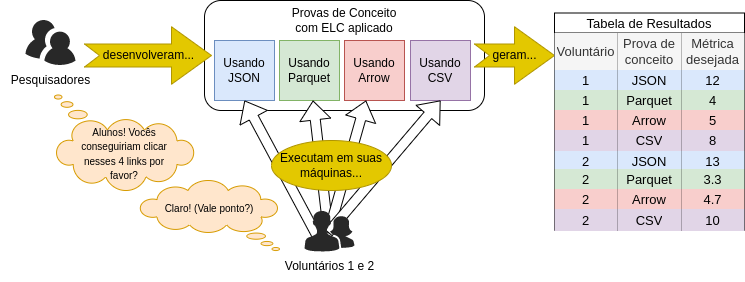
\includegraphics[width=0.9\textwidth]{figures/exemplo-tipo-de-dado.png}
		\caption{Exemplo de como seria o cenário da pesquisa sobre o tráfego de dados usando o \acr{ELC}.}
		\label{fig:exemplo-tipo-de-dado}
	\end{figure}

	A contribuição principal do \acr{ELC} é oferecer uma abordagem prática para realizar a execução de tarefas customizáveis no lado do cliente, e também o registro dos resultados dessas execuções em uma base de dados, também customizável, para análise. Dessa forma, seria possível resolver o problema da equipe sem muitas complicações. 

	Ademais, o \emph{framework} por padrão possui algumas métricas básicas implementadas, como tempo gasto na tarefa, memória utilizada e a identificação do ambiente de execução, e os dados são armazenados em uma planilha online para fácil obtenção e análise. Deste modo, o desenvolvedor tem uma base pronta para estender, e pode focar nas provas de conceito e na obtenção de ambientes e voluntários para seus testes, ao invés do desenvolvimento de infraestrutura para realização e registro das medições.

	Porém, existem algumas limitações com relação a ferramenta que precisam ser levadas em consideração antes do seu uso. Atualmente, somente métricas e dados em execução conseguem ser coletados pela ferramenta, ou seja, ainda não é possível realizar testes de caixa branca \footnote{Sobre testes de caixa branca: \citep[Capítulo 21]{Sommerville2015Software}}. Além disso, não são contempladas por padrão métricas de renderização, como o tempo de carregamento de páginas, já que existem outras ferramentas que abordam esse tipo de medição, como a WePR, mencionada na seção \ref{WePR}.

	O trabalho está organizado da seguinte forma: O capítulo \ref{cap:fundamentacao_teorica} corresponde à fundamentação teórica do projeto. O capítulo \ref{cap:metodologiatrabsrelacionados} corresponde à metodologia utilizada na pesquisa dos trabalhos relacionados e contém também os principais trabalhos relacionados encontrados. O capítulo \ref{cap:implementação} apresenta a proposta de desenvolvimento da ferramenta. O capítulo \ref{cap:experimentos} apresenta os experimentos realizados utilizando a ferramenta e seus resultados, e por fim o capítulo \ref{cap:conclusão} traz a conclusão do projeto.


\chapter{Fundamentação teórica}
	\label{cap:fundamentacao_teorica}

		Neste capítulo será apresentada a fundamentação teórica do trabalho, ou seja, os principais conceitos teóricos a serem utilizados no entendimento da construção e do uso do \acr{ELC}. Dessa forma, a primeira seção trata de Testes de Software, a segunda sobre Abordagem Empírica em Engenharia de Software, a terceira sobre Padrões de Projeto (os utilizados no projeto foram o Strategy e o Composite), a quarta do princípio do Aberto-Fechado e a última sobre Coesão e Acoplamento.

		\section{Testes de Software}
		\label{cap:software-testing}
		O desenvolvimento de software é uma atividade propensa a erros humanos, que podem ser introduzidos em várias etapas do processo.
		Para mitigar essa característica inerente, a área de testes de software surgiu como um componente crítico da engenharia de software, no âmbito da garantia de qualidade de software.
		O principal objetivo dos testes de software é identificar e corrigir o maior número possível de erros antes da entrega do software ao cliente.
		Isso é realizado por meio da criação de uma série de casos de teste que, utilizando técnicas específicas de teste de software, exercitam o software com alta probabilidade de encontrar erros \citep{pressman2009software}.

		Os testes de software desempenham um papel fundamental na garantia de qualidade de software, uma vez que suas outras atividades não são, por si só, suficientes na detecção e correção de erros.
		Isso ocorre porque, sempre que um programa é executado, ele está, de fato, passando por um processo de teste.
		Portanto, a extensa aplicação de testes é necessária para identificar e solucionar erros antes que o software chegue às mãos do cliente \citep{pressman2009software}.

		Os testes de software podem ser classificados em dois tipos principais: testes de caixa branca e testes de caixa preta.
		No caso dos testes de caixa branca, o conhecimento das estruturas internas do software é utilizado para projetar os casos de teste.
		Em contrapartida, os testes de caixa preta se concentram em exercitar os requisitos do software, ignorando sua estrutura interna. Esses testes avaliam o que o software faz, sem se preocupar com como ele faz \citep{pressman2009software}.

		Dentro do contexto de um framework de análise de consumo de recursos computacionais de aplicações web do lado cliente, a escolha dos tipos de teste a serem realizados é crucial.
		O \acr{ELC} é primariamente focado na análise do consumo de recursos computacionais, sem acoplamento com o funcionamento interno do software testado.
		Portanto, os casos de teste de caixa preta são os mais apropriados.
		No entanto, é importante destacar que, devido à capacidade do ELC de permitir análises compostas, por meio da árvore de tarefas \ref{task-tree}, ele também pode oferecer algum nível de visibilidade das estruturas internas do objeto de teste.


		\section{Abordagem Empírica em Engenharia de Software}
		\label{cap:engenharia-de-software-empirica}

		A engenharia de software é um campo multidisciplinar. Abrange desde tópicos técnicos, como bancos de dados e sistemas operacionais, até questões relacionadas a linguagens de programação, como sintaxe e semântica, e até temas sociais e  psicologia. O desenvolvimento de software é humano; esse que é até hoje incapacitado de criar um código completamente do zero. É uma disciplina baseada em criatividade, e na ingenuidade das pessoas trabalhando na área. \citep{wohlin2012experimentation}.

		Em contraponto, é necessário, quando estudando ou fazendo pesquisas no campo, mirar em tratá-la como uma disciplina científica. Ou seja, utilizar métodos científicos para realizar as pesquisas, e também na hora de tomar decisões sobre mudanças na forma com a qual é feito o desenvolvimento. Para isso, é preciso entender os métodos que estão disponíveis para serem utilizados, suas limitações e quando eles devem ser aplicados \citep{wohlin2012experimentation}. Isso também deve ser aplicado na hora de escolher as ferramentas para o desenvolvimento das aplicações.

		Nesse contexto, o \acr{ELC} fornece insumos úteis aos pesquisadores e desenvolvedores na hora de avaliar essas ferramentas, pois permite estabelecer critérios objetivos na hora de comparar abordagens no desenvolvimento de aplicações web.

		\section{Padrões de Projeto}
		\label{cap:padroes-de-projeto}

		Os Padrões de Projeto dão nome, abstraem e identificam os aspectos comuns da construção de uma estrutura, e são úteis para implementar uma abordagem orientada a objetos reutilizável em aplicações. Eles identificam as instâncias e classes, seus papéis e colaborações e a distribuição de responsabilidades na implementação. Cada padrão foca em um problema específico de projeto já abordado e provado, tornando acessível aos desenvolvedores de novos sistemas soluções úteis na construção de uma implementação reutilizável \citep{gamma1994design}.
		
		Existem diversos padrões de projeto diferentes, como descritos no livro de \cite{gamma1994design}. Os padrões utilizados na implementação do \acr{ELC} foram o Composite e o Strategy.

		\subsection{Composite}
		\label{subsection:composite}

		O padrão de projeto Composite é utilizado quando é desejado representar uma hierarquia de objetos, e o objetivo é fazer com que o cliente ignore as diferenças entre os objetos compostos e os individuais, interagindo da mesma maneira nos dois casos. Como consequência, esse padrão faz com que o cliente seja simples. Como os objetos são tratados da mesma maneira, o código do cliente acaba ficando mais simples \citep[Capítulo 4]{gamma1994design}.
		
		Além disso, o uso do padrão torna fácil a adição de novos tipos de componentes, basta implementar a classe que o cliente entende. Dessa forma, os clientes não precisam ser alterados caso os objetos sejam modificados. Uma desvantagem desse padrão é que torna a validação dos componentes mais complicada, pois não se pode contar plenamente com a tipagem para garantir os requisitos dos dados. São necessárias validações em tempo de execução \citep[Capítulo 4]{gamma1994design}. Esse padrão foi utilizado na construção das tarefas, processo descrito na seção \ref{subsection:modulo-tasks}.

		\subsection{Strategy}
		\label{subsection:strategy}

		O padrão de projeto Strategy é ideal para ser utilizado quando muitas classes diferem somente no seu comportamento, ou são desejadas diferentes variações de um mesmo algoritmo. Dessa forma, é possível definir a implementação de cada uma das variações mantendo a mesma estrutura para a aplicação \citep{gamma1994design}. 

		Essa abordagem faz com que diminua o uso de condições que gerenciam o comportamento do algoritmo na classe principal, abstraindo essa lógica para dentro do Strategy. Assim, esse tipo de lógica mais específica do comportamento da classe fica oculta da classe principal, tornando mais simples de ser entendida  \citep{gamma1994design}. O padrão Strategy foi utilizado na construção do site utilizado no exemplo descrito na seção \ref{subsection:study-case-easyelc}, na implementação dos diferentes algoritmos para o cálculo de números primos.


		\section{Princípio do Aberto/Fechado}
		\label{cap:solid-ocp}
		\citet{MartinCleanArchtecture2017} popularizou os princípios de design de software SOLID.
		Os quais atuam como guias na organização de funções e estruturas de dados em classes e como essas classes devem ser interconectadas.
		Outro ponto importante, é que esses princípios são pensados para serem aplicados por programadores que trabalham no nível do módulo.
		Ou seja, sua aplicação ocorre um nível de abstração acima do código e visa definir os tipos de estruturas usadas dentro de módulos e componentes.
		O principal objetivo dos princípios SOLID é a criação de estruturas de software que tolerem mudanças, sejam fáceis de entender e sejam a base de componentes reutilizáveis em diferentes sistemas de software.

		O princípio do aberto/fechado (do inglês, \emph{open/closed principle} ou OCP) pode ser definido como um artefato de software deve ser aberto para extensão, mas fechado para modificação. \citep{Meyer1997ObjectOrientedSoftwareConstruction}
		Em outras palavras, podemos afirmar que o princípio não foi respeitado quando uma extensão simples de um requisito resulta em uma cascata de mudanças em módulos dependentes.
		O \acr{OCP} provoca justamente neste ponto, onde idealmente os módulos nunca são alterados.
		Deste modo, quando houver a extensão de algum requisito, a extensão no software é feita adicionando código novo, ao invés de, alterar o código existente que funciona. \citep{Martin2000TheOP}

		O \acr{OCP} é reconhecido como o coração do design de classes e módulos por estudantes de design de software. \citep{MartinCleanArchtecture2017}
		Pois, permite que mudanças aconteçam sem que haja um grande impacto no software.
		E, atinge este objetivo por meio do particionamento do sistema em componentes, organizando eles em uma hierarquia de dependência a qual protege os componentes de nível mais alto das mudanças no componentes de nível mais baixo. \citep{MartinCleanArchtecture2017}

		A arquitetura do framework ELC utiliza como principal guia o \acr{OCP}.
		Pois, organizamos os módulos do framework como entidades completamente independentes, assegurando que qualquer referência intermodular deveria ser feita para a interface do módulo.
		Desta forma, o risco de alguma mudança em um módulo resultar em alterações em outro módulo é minimizado e permite que múltiplos módulos sejam desenvolvidos em paralelo sem haver retrabalho.
		Ademais, definimos os módulos do \acr{ELC} como os pontos de extensão do framework.
		Ou seja, cada módulo é projetado para caso alguma mudança de comportamento seja necessária, a alteração é incluída criando uma nova classe a qual estende a interface do módulo.

		\section{Coesão e Acoplamento}
		\label{section:coesao-e-acoplamento}

		Coesão implica que um componente ou classe encapsule somente atributos e operações que são relacionadas diretamente entre si ou a própria classe ou componente. Na engenharia de software são definidos diversos tipos, dentre eles \citep{pressman2009software}:

		\begin{enumerate}
			\item Coesão funcional: demonstrada primariamente por operações, esse nível de coesão ocorre quando um componente executa uma operação e retorna um resultado.
			\item Coesão de camadas: Demonstrada nos pacotes, componentes e classes, esse tipo de coesão ocorre quando uma camada superior da arquitetura acessa os serviços de uma camada inferior, mas o contrário não é possível.
			\item Coesão comunicacional: Todas as operações que acessam o mesmo dado são definidas em uma única classe. No geral, essas classes focam primariamente no dado em sí, o acessando e armazenando.
		\end{enumerate}

		Classes e componentes que exibem esses três níveis de coesão são relativamente fáceis de implementar, testar e manter. Esse deve ser um objetivo na hora do desenvolvimento de software \citep{pressman2009software}.
		
		Conforme o nível de comunicação e colaboração cresce, a complexidade do sistema também cresce. Isso gera dificuldades na implementação, testes e na manutenção do software. Acoplamento é uma medida de qualidade que quantifica o nível no qual as classes estão conectadas entre si. Conforme as classes e componentes se tornam mais dependentes uns dos outros, o acoplamento cresce. Um objetivo importante no projeto de uma arquitetura é manter o acoplamento o mais baixo possível \citep{pressman2009software}.

		Esse critério é importantíssimo quando se avalia a escolha de uma ferramenta para medição no lado do cliente, pois quanto mais acoplada a ferramenta for à implementação do problema, mais difícil e demorada será sua utilização. No desenvolvimento do \acr{ELC}, foram considerados esses padrões de qualidade, tanto no desenvolvimento da arquitetura de módulos, como explicado na seção \ref{cap:arquitetura}, quanto na implementação das classes internas da aplicação. 


\chapter{Trabalhos Relacionados}
	\label{cap:metodologiatrabsrelacionados}

	\par Tendo em vista os principais conceitos que fundamentam o trabalho, neste capítulo estão descritas as principais ferramentas encontradas dentro do campo de medição no lado do cliente. Na seção \ref{section:metodologia-de-pesquisa}, é descrita a metodologia utilizada para a obtenção dos principais trabalhos relacionados. A seção \ref{sec:ferramentas-medicao-clientside} contém, além do estabelecimento de uma série de critérios objetivos para analisar as ferramentas encontradas, é realizado um resumo de cada ferramenta e sua análise. Por fim, é feita uma relação dos trabalhos já classificados, na seção \ref{section:analise-ferramentas}.

	\section{Metodologia de Pesquisa}
	\label{section:metodologia-de-pesquisa}

	Para a revisão bibliográfica as duas principais ferramentas utilizadas foram: Elicit, um assistente de pesquisa baseado em modelos de transformador pré-treinado generativo (do inglês, \emph{generative pre-trained transformer}) de aprendizado de máquina, e a ferramenta Connected Papers, a qual  gera um grafo de artigos relacionados baseado em cocitações e acoplamento bibliográfico.
	A ferramenta Elicit funciona recebendo uma pergunta em linguagem natural e retornando os trabalhos que considera mais relevantes, junto a um resumo, em uma tabela paginada.
	Deste modo, na tabela \ref{tab:strings-elicit} elencamos todas strings de busca utilizadas no Elicit, e para cada uma delas consultamos até a segunda página da tabela, totalizando 14 trabalhos retornados por string de busca.

	\begin{table}[H]
	\centering
	\caption{Strings utilizadas na ferramenta Elicit para encontrar trabalhos relacionados.\label{long}}
		\begin{tabular}{||c||} 
			
		\hline
			Strings de Busca \\
		\hline\hline
		``browsing memory'' \\
		``client side memory performance'' \\
		``client side memory profiling'' \\
		``memory network management web client'' \\
		``memory network performance web client'' \\
		``memory network profiling web client'' \\
		``memory network waste web client'' \\
		``measuring performance in client side'' \\
		``measuring in client side'' \\
		``performance measurement'' \\
		``tools to measure performance in client side'' \\
		``evaluating latency on client side'' \\
		``optimizing web browsing'' \\
		``performance tool web client side'' \\
		``waste resources client side'' \\
		``waste resources web client'' \\
		``web client side memory performance'' \\
		``What are the impacts of memory management in mobile Web Browsing?'' \\
		``What is the state-of-the-art for measuring performance of client side?'' \\
		``What is the state-of-the-art for measuring QoE and memory of Web Browsing?'' \\

		\hline
		\end{tabular}
	\label{tab:strings-elicit}
	\end{table}

	Além disso, três trabalhos encontrados por meio do Elicit foram utilizados como entrada para a ferramenta Connected Papers. O Connected Papers é um outro assistente de pesquisa, o qual recebe como entrada o título ou o DOI de um trabalho para gerar um grafo de trabalhos relacionados destacando suas principais conexões e trabalhos influentes.	Na tabela \ref{tab:strings-connected-papers} estão listadas as strings de busca utilizadas no Connected Papers, de modo que, para cada uma, a ferramenta gerou um grafo com 40 trabalhos relacionados, os quais também podem ser visualizados em uma tabela.

	\begin{table}[H]
	\centering
	\caption{Strings utilizadas na ferramenta Connected Papers para encontrar trabalhos relacionados.}
		\begin{tabular}{||c||} 

		\hline
			Strings de Busca \\
		\hline\hline
		``Measuring Web Latency and Rendering Performance: Method, Tools, and Longitudinal Dataset''\\
		``MemInsight: platform-independent memory debugging for JavaScript''\\
		``Obtaining in-context measurements of cellular network performance''\\
		\hline
		\end{tabular}
		\label{tab:strings-connected-papers}
	\end{table}

	Na tabela \ref{tab:trabalhos-encontrados} constam os resultados da pesquisa bibliográfica no estado da arte. No total foram 400 trabalhos relacionados pré selecionados, e foram selecionados 4 trabalhos contendo ferramentas relevantes no tema proposto, a serem apresentados na próxima seção. 

	\begin{table}[H]
		\centering
		\caption{Total de trabalhos encontrados utilizando as ferramentas Elicit e Connected Papers}
		\begin{tabular}{l  c L{1.5cm} R{1.5cm}}
			\toprule
			\textbf{Ferramenta} & \textbf{Trabalhos Encontrados} \\
			\midrule
			Elicit  &  280  \\
			Connected Papers  &  120  \\
			\midrule
			Total  &  400  \\
			\bottomrule
		\end{tabular}
		\label{tab:trabalhos-encontrados}
	\end{table}


	Os critérios usados para filtrar os trabalhos encontrados por meio de ambas as ferramentas estão descritos na figura \ref{fig:fluxo-leitura}. Em suma, após a leitura do resumo de cada trabalho, três critérios foram avaliados, sendo cada um deles um dos filtros. Os critérios foram: Se o trabalho não teria relação suficiente com o tema, se é necessário ler a introdução para a tomada da decisão ou se é um trabalho o qual a leitura completa deve ser realizada.

	\begin{figure}[H]
		\centering
		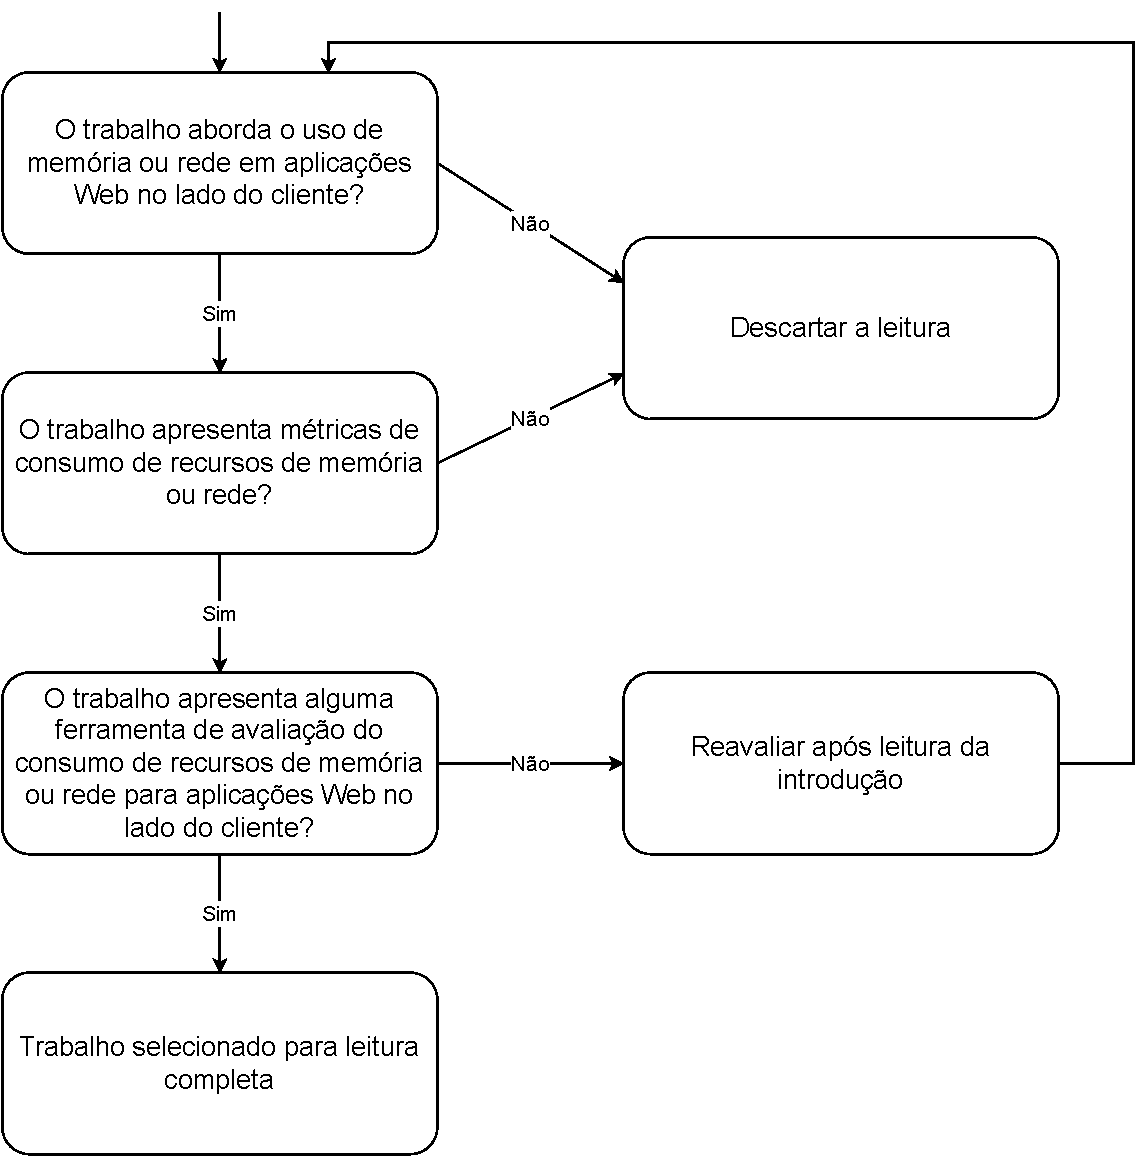
\includegraphics[width=0.6\textwidth]{figures/fluxo-decisao-leitura.pdf}
		\caption{Fluxo dos critérios utilizados para seleção dos trabalhos relacionados para leitura.}
		\label{fig:fluxo-leitura}
	\end{figure}

	\section{Ferramentas Para Medição no Lado do Cliente}
	\label{sec:ferramentas-medicao-clientside}

	Após a leitura dos principais trabalhos, conseguimos obter uma visão abrangente das ferramentas e soluções existentes e propostas no âmbito acadêmico. Com isso, foi efetuada uma categorização dessas ferramentas com base em uma série de parâmetros, explicitados na tabela \ref{tab:criterio-avaliacao-ferramentas}, e com o objetivo de avaliar o quão complementar é o \acr{ELC} em relação ao estado da arte.

	\begin{table}[H]
		\centering
		\caption{Critérios de classificação para as ferramentas de medição no lado do cliente}
		\begin{tabular}{lp{8.5cm}}
			\toprule
			\textbf{Critério} & \textbf{Descrição}\\
			\midrule 
			Coesão e Acoplamento & Se a utilização da ferramenta exige que o código fonte seja pouco alterado.\\
			Extensibilidade & Se a ferramenta permite a coleta de métricas customizáveis.\\
			Portabilidade & Se a ferramenta pode ser utilizada em testes multiplataforma.\\
			Armazenamento em Nuvem & Se a ferramenta gera dados estruturados para análise futura.\\
			\bottomrule
		\end{tabular}
		\label{tab:criterio-avaliacao-ferramentas}
	\end{table}

	O critério de Coesão e Acoplamento é importante na avaliação das ferramentas pois facilita na utilização, diminuindo a dificuldade e complexidade na implementação da ferramenta. No exemplo dos pesquisadores, explicado no capítulo \ref{cap:intro}, é desejado que não seja necessário alterar, por exemplo, o código das provas de conceito a serem executadas no experimento. 
	
	O segundo critério citado, Extensibilidade, é importante pois, dado o universo de métricas e tarefas possíveis dentro de um experimento, habilita ao pesquisador representar seu problema da maneira mais fiel, inclusive com cenários customizados. Assim, uma boa extensibilidade permite que existam tarefas simples e complexas, configurando diferentes cenários de testes.
	
	Já o critério de Portabilidade é essencial pois o ambiente da \emph{web} moderna é diverso, contendo diferentes plataformas e dispositivos, e a possibilidade de testar o desempenho de um método em diferentes ambientes traz mais solidez para os resultados da pesquisa. No contexto dos pesquisadores, é necessário que a ferramenta a ser utilizada realize os testes em diversas plataformas.
	
	E o último critério que foi destacado, o de Armazenamento em Nuvem, é um grande facilitador para o trabalho de análise posterior, que poderá utilizar esses dados centralizados de forma remota e simplificada, apenas consumindo uma planilha ou obtendo os dados via banco de dados pela internet.

	\subsection{MemInsight}
	\label{subsection:meminsight}

	No contexto de medição de memória, temos o MemInsight \citep{Jensen2015MemInsight}. Essa ferramenta roda de forma independente sobre um motor Javascript, não sendo necessário um navegador para executá-la, e faz a análise do consumo de memória por meio de um conjunto de medições que visam remontar o ciclo de vida dos objetos em memória, e que permitem a análise de desperdício de recursos durante a execução do programa. 

	Para a implementação da ferramenta, não são necessárias alterações no código fonte, visto que ela opera sobre os nós do \acr{DOM}, atendendo dessa forma ao critério de Coesão e Acoplamento. É possível executar a ferramenta sob qualquer motor Javascript, seja um navegador de \emph{Desktop} ou em celulares, até em servidores utilizando NodeJS. Portanto, atende ao critério de Portabilidade.


	É observável que a ferramenta só trabalha com medição de métricas de memória, não permitindo generalizar consultas de outros tipos, por isso não atende ao critério de Extensibilidade. Além disso, por ser uma ferramenta com foco em depurar aplicações, não realiza nativamente a persistência e organização desses dados, não atendendo ao critério de Armazenamento em Nuvem.		

	\subsection{WePR}
	\label{WePR}
	\par \citet{Asrese2019MeasuringWL} também propôs uma ferramenta para medição no lado do cliente, porém com o foco em métricas de \acr{QoS}, nomeada WePR. A ferramenta é distribuída, e consiste basicamente de um coletor, um servidor que fornece os elementos das páginas para medição, múltiplos servidores de renderização gerenciados por um balanceador de carga (do inglês, \emph{load balancer}), e um servidor que cuida da persistência dos dados. Dessa forma, o coletor inicialmente pede ao servidor as URLs dos elementos a serem medidos, e após obter essa resposta, faz o download desses elementos e captura métricas. Posteriormente, envia esses dados medidos e os elementos baixados para o balanceador de carga, e por fim algum dos servidores de renderização envia os dados para persistência. 

	A ferramenta é orientada à medição de websites e páginas na web, e interage com essas páginas via requisições do tipo \acr{HTTP}. Dessa forma, atende ao critério de Coesão e Acoplamento, pois não exige que o código fonte seja modificado para o seu uso, mas não atende ao critério de Portabilidade, pois é utilizada somente para o contexto de websites.

	Como a ferramenta realiza a persistência de dados de forma remota, atende ao critério de Armazenamento em Nuvem. Em contrapartida, a ferramenta é capaz de lidar somente com métricas de \acr{QoS}, não sendo possível customizar métricas, e por isso não atende ao critério de Extensibilidade.

	\subsection{Gember}
	\par \citet{Gember2012Obtaining} também traz um estudo sobre medição no lado do cliente, porém dessa vez em clientes móveis, buscando medir o desempenho de rede desses aparelhos em um período de tempo. Foi desenvolvido no trabalho um protótipo para Android de um medidor de performance para analisar somente quando o dispositivo está ativo. A arquitetura da ferramenta consiste basicamente de um controlador central (servidor), e múltiplos clientes (aparelhos) com o medidor instalado e rodando em seus celulares. Dessa forma, o pesquisador faz uma requisição para esse controlador, e ele coordena a coleta do que foi solicitado nos aparelhos, salvando os resultados no servidor.

	O serviço inicialmente coleta latência, taxa de transferência (do inglês, \emph{throughput}) e o tempo de carregamento de páginas Web, e é extensível para outras métricas de rede, porém limitado a elas. Isso torna a ferramenta insuficiente no critério de Extensibilidade, pois não é possível coletar métricas customizadas. 

	Com relação ao seu uso, não é necessário modificar o código das aplicações que utilizam a rede celular para as medições, visto que o medidor é uma aplicação apartada instalada no aparelho do cliente. Isso faz com que a ferramenta satisfaça o critério de Coesão e Acoplamento. 

	Os dados coletados são persistidos no próprio servidor remoto que coordena as coletas, o que atende ao critério de Armazenamento em Nuvem. Porém, uma limitação da ferramenta é a utilização somente em clientes Android, tornando pouco flexível o seu uso em contextos de pesquisas multiplataforma, e fazendo com que a ferramenta não atenda ao critério de Portabilidade.

	\subsection{Mobilyzer}
	\par Ainda no contexto de medição de rede, se encontra o Mobilyzer \citep{Nikravesh2015Mobilyzer}, uma plataforma aberta para medição de rede em dispositivos móveis. Essa plataforma foi criada com o objetivo de prover uma solução escalável, eficiente e controlável, que fosse possível de ser incorporada tanto a apps em desenvolvimento, quanto em apps que já estão desenvolvidos, para suportar pesquisas e testes em medição de rede. 
	\par Ela funciona utilizando alguns componentes básicos, sendo eles: 
	\begin{enumerate}
		\item Uma biblioteca Android, que é integrada aos aplicativos para coletar as informações e enviar ao servidor. Ela é incorporada direto no código fonte das aplicações.
		\item Um componente chamado gerenciador de memória, no qual o pesquisador pode inserir medições de forma customizada e mais eficiente. Ele também realiza o agendamento das medições, e também coordena e monitora os dispositivos para que não tenha sobrecarga em nenhum aparelho ou rede medida. 
		\item Um servidor na nuvem, que fica responsável por coletar, analisar aplicando regras e publicar os dados coletados dos dispositivos. Essa arquitetura centralizada simplifica o compartilhamento de dados entre essas etapas, podendo integrar outras ferramentas de análise de dados com a base das coletas.

	\end{enumerate}

	A utilização da biblioteca Android nos aplicativos não exige muitas alterações no código fonte das aplicações, bastando apenas instalar a biblioteca e adicionar as chamadas a \acr{API} do gerenciador de memória rodando no aparelho. Isso torna a ferramenta apta no critério Coesão e Acoplamento, já que são poucas alterações no código fonte. Com relação a persistência, o servidor na nuvem mantém uma base de dados anonimizada com os resultados das medições para consulta, tornando a ferramenta apta no critério de Armazenamento em Nuvem.

	Uma limitação no uso do Mobilyzer em pesquisas é que essa plataforma também se restringe a plataforma Android, não atendendo ao critério de Portabilidade. Além disso, não possui muita flexibilidade com relação às métricas, sendo em sua maior parte métricas de rede, e por isso não atende ao critério de Extensibilidade.
		
	\section{Classificação das ferramentas}
	\label{section:analise-ferramentas}
	Após a análise individual de cada ferramenta, foi possível representar suas classificações dados os critérios definidos anteriormente. Esse processo está exemplificado na tabela \ref{table:classificacao-sem-elc}. Essa análise foi importante para entender aonde o \acr{ELC} se encaixa no panorama geral das ferramentas de medição no lado do cliente.

	\begin{table}[ht]
	\caption{Classificação das ferramentas encontradas} % title of Table
	\centering % used for centering table
	\begin{tabular}{c c c c c } % centered columns (4 columns)
	\toprule %inserts double horizontal lines

	\textbf{Ferramentas} &\textbf{MemInsight} & \textbf{WePR} & \textbf{Gember} & \textbf{Mobilyzer}  \\ [0.4ex]

	%heading
	\midrule % inserts single horizontal line
	Coesão e Acoplamento & \cmark & \cmark & \cmark & \cmark   \\
	Extensibilidade & \xmark & \xmark & \xmark & \xmark  \\
	Portabilidade & \cmark & \xmark & \xmark & \xmark  \\
	Armazenamento em núvem & \xmark & \cmark & \cmark & \cmark  \\
	\bottomrule %inserts single line
	\end{tabular}
	\label{table:classificacao-sem-elc} % is used to refer this table in the text
	\end{table}
\chapter{Implementação}
	\label{cap:implementação}

	% TO-DO: Melhorar fluidez do texto. Quando mostrar código, integrar ele no texto. 

	Neste capítulo, abordamos os aspectos relacionados à implementação da ferramenta, incluindo sua concepção e arquitetura interna.
	Inicialmente, apresentamos estudos de caso \ref{sec:estudos-de-caso} que exemplificam o uso da ferramenta.
	Em seguida, exploramos os detalhes de implementação, que incluem diagramas de arquitetura \ref{cap:arquitetura} e a construção interna de cada módulo a partir da subseção \ref{subsection:modulo-project} até a \ref{subsec:implemencao-easyelc}.

	\section{Estudos de Caso}
	\label{sec:estudos-de-caso}

	Para fins didáticos, estão descritos nesta seção dois estudos de caso, os quais ilustram os possíveis fluxos de uso da ferramenta.
	A subseção \ref{subsection:study-case-cloning-elc} exemplifica o uso do \acr{ELC} a partir de um clone de seu repositório.
	Enquanto, a subseção \ref{subsection:study-case-easyelc} exemplifica o uso da ferramenta como uma biblioteca. 
	Em ambos cenários, utilizamos o mesmo objeto de estudo, uma avaliação empírica de funções que calculam se um número é primo.
	O racional por trás deste exemplo consiste em sua facilidade de explicação, sua adaptação a ambos os fluxos de uso e na alta probabilidade de os usuários do \acr{ELC}, notadamente programadores, terem tido algum contato com problemas semelhantes durante sua formação.

	Então, considere haver uma pesquisa onde são comparadas diferentes funções para gerar listas contendo os primeiros $n$ números primos. 
	Deseja-se, de forma empírica, obter qual função em média leva menos tempo para calcular as listas de números primos em múltiplos tipos de hardware.
	Para isso, é necessário executar as funções, obter o tempo de execução para cada tamanho de lista testado e centralizar os resultados obtidos, a fim de concluir qual função é mais eficiente.
	O meio para realizar esta avaliação será um site estático, o qual pode ser facilmente gerado a partir do repositório do \acr{ELC}.

	\subsection{Uso do ELC a partir de um Clone do Repositório}
	\label{subsection:study-case-cloning-elc}

	Para realizar o experimento do cálculo dos números primos utilizando o \acr{ELC}, uma das opções é realizando um clone de seu repositório no GitHub\footnote{\url{https://github.com/El-Chupacabra-TCC/el-chupacabra}}.
	Após isso, para cada algoritmo que se deseja avaliar, é necessário implementar uma classe herdeira de \emph{BaseTask}, onde o método \emph{execute} encapsula o algoritmo.

	A listagem \ref{lst:elc_firstnprimes_task} contém um exemplo de classe base para as funções de calcular números primos.
	O tamanho da lista é definida via construtor e armazenado na variável de instância \emph{howMany}.
	Enquando, o método \emph{execute} contém um laço na linha 13 que preenche a lista com números primos detectados pelo método \emph{isPrime}.
	Este que, por sua vez, pode ser sobrescrito nas subclasses para conter a implementação de cada função que o experimento avalie.

\begin{lstlisting}[label={lst:elc_firstnprimes_task}, caption={Exemplo de classe encapulando um algoritmo de cálculo de números primos.}, language=TypeScript, breaklines=true]
export default class FirstNPrimesTask extends BaseTask {
  protected howMany: number

  constructor(metrics: IMetric[], howMany: number) {
    super(metrics)
    this.howMany = howMany
  }

  protected async execute(): Promise<Record<string, any>> {
    const results = { amountOfPrimes: 0, primes: [] }
    const primes: number[] = []

    for (let i = 0; primes.length < this.howMany; i++) {
      if (this.isPrime(i)) {
        primes.push(i)
      }
    }

    results.primes = primes
    results.amountOfPrimes = primes.length
    return results
  }

  protected isPrime(i: number): boolean {
    // ...
    return true
  }
}
\end{lstlisting}

	Com uma classe para cada algoritmo em avaliação, o próximo passo é criar um script principal para a execução das avaliações.
	O repositório já contém um arquivo Index.ts como exemplo de script principal para avaliações executadas em navegadores.
	Partindo dele como base, é necessário realizar quatro configurações:

	\begin{itemize}
		\item Perfil do ambiente de execução: As avaliações usando o \acr{ELC} podem ser executadas em diferentes tipos ambientes.
		Para que seja possível coletar informações sobre o ambiente que a avaliação está sendo executada é necessário utilizar uma instância de perfil de execução adequada.
		Na listagem \ref{lst:elc_index_ts_example}, na linha 3 instanciamos o perfil de execução para navegadores.

		\item Persistência das métricas: Define onde os dados coletados pelo \acr{ELC} são armazenados.
		Na listagem \ref{lst:elc_index_ts_example}, consideramos que as métricas coletadas devem ser enviadas para uma planilha no Google Sheets.
		Deste modo, mesmo executando a avaliação em múltiplos ambientes, os dados coletados são armazenado em um único lugar.
		Para tal, na linha 4 instanciamos o \emph{SheetsonPersister} com configurações de qual planilha usar e um token de autenticação.

		\item Árvore de tarefas: Tarefa é o nome dado às classes que são a carga sob avaliação do \acr{ELC} e entre as linhas 10 e 16 da listagem \ref{lst:elc_index_ts_example} há a construção de uma árvore de tarefas.
		Utilizamos o \emph{CompositeTask} como raíz da árvore, o qual tem como papel agrupar outras tarefas, além de receber uma lista de métricas para avaliar o grupo que engloba.
		Nas linhas 14 e 15, são definidas duas instâncias da classe \emph{FirstNPrimesTask}, pois a primeira é uma avaliação para o tamanho de lista $10000$ e a segunda $30000$, ademais \emph{DeltaTimeMetric} será a única métrica coletada individualmente.

		\item Métricas em uso: Cada instância de tarefa possui como primeiro argumento uma lista de métricas, como podemos observar nas linhas 11, 13 e 14 da listagem \ref{lst:elc_index_ts_example}.
		Deste modo, cada instância de tarefa possui um conjunto independente de métricas.
		Por outro lado, métricas podem ser coletadas sobre um conjunto de tarefas quando este é agrupado por uma \emph{CompositeTask} como é o caso das métricas na linha 11.
	\end{itemize}

\begin{minipage}{\linewidth}
\begin{lstlisting}[label={lst:elc_index_ts_example}, caption={Exemplo de script principal avaliando uma comparação de tempo de execução entre duas execuções de uma tarefa FirstNPrimesTask. Onde a avaliação é executada em navegadores e as métricas coletadas são armazenadas em uma planilha online.}, language=TypeScript, breaklines=true]
export function Execute()
{
  const executionProfile = new BrowserExecutionProfile();
  const persister = new SheetsonPersister(
    "SHEET_NAME",
    "API_KEY",
    "SHEET_ID"
  );

  const tasks = new CompositeTask(
    [new MemoryMetric(), new DeltaTimeMetric()],
    [
      new FirstNPrimesTask([new DeltaTimeMetric()], 10000),
      new FirstNPrimesTask([new DeltaTimeMetric()], 30000)
    ]
  );

  var project = new Project(executionProfile, tasks, [persister]);
  return project.executeTask();
}
\end{lstlisting}
\end{minipage}

	Após isso, somos capazes de criar uma instância de Project utilizando as configurações como argumentos de seu construtor.
	E, a avaliação será executada quando o método executeTask da instância de Project for invocado.
	Como último passo, utilizamos o compilador do TypeScript para gerar os arquivos JavaScript e hospedar o artefato gerado em algum servidor Web.
	Se o artefato for gerado com o código padrão do repositório, ele será um site estático com um botão para executar a avaliação como ilustra a figura \ref{fig:elc_clone_artifact}.

	\begin{figure}[!ht]
		\centering
		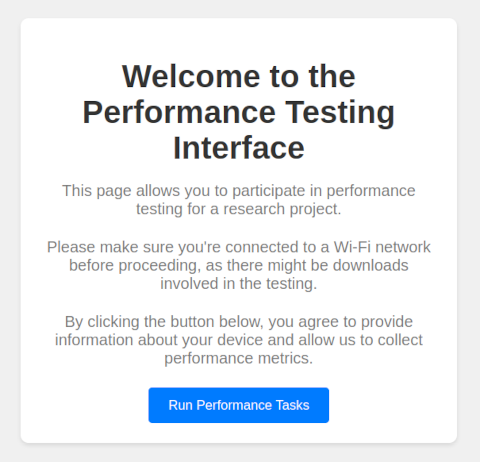
\includegraphics[width=0.6\textwidth]{figures/elc-clone-artifact.png}
		\caption{Página HTML padrão gerada como artefato para avaliações do ELC no fluxo de uso por clone do repositório. Ela contém um botão o qual inicia a execução das tarefas e a coleta das métricas.}
		\label{fig:elc_clone_artifact}
	\end{figure}

	\subsection{Uso do ELC por meio da Interface EasyElc}
	\label{subsection:study-case-easyelc}

	Nesta seção o \acr{ELC} é utilizado como uma dependência de um projeto em ambiente produtivo.
	Considere o cenário de um site estático que realiza o cálculo da lista de números primos no navegador do usuário.
	Este site possui mais de um algoritmo para o cálculo dos números primos e seu usuário pode escolher qual quer utilizar.
	E, para coletar métricas das execuções dos algoritmos, o \acr{ELC} é utilizado.

	% TO-DO: Criar um apêndice detalhado sobre o First n Primes Calculator.

	Com o propósito de exercitar este exato cenário, desenvolvemos o site Calculadora dos Primeiros n Números Primos (do inglês, \emph{First n Primes Calculator})
	\footnote{\url{https://el-chupacabra-tcc.github.io/FirstNPrimes}}.
	Onde o usuário insere o tamanho da lista de números primos que deseja e o site calcula a sequência dos números primos do 2 até a quantidade solicitada.
	Porém, o site sempre recalcula a sequência dos números primos, não conta com qualquer mecanismo de cache, e usando os recursos da máquina do usuário.

	\begin{figure}[!ht]
		\centering
		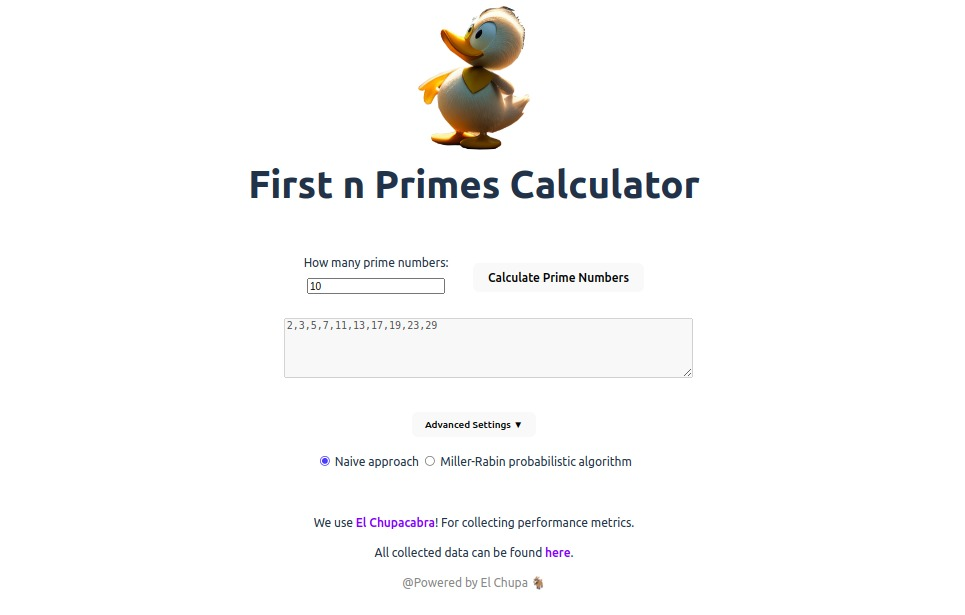
\includegraphics[width=1\textwidth]{figures/print-elc-numeros-primos.jpeg}
		\caption{Impressão de tela do site Calculadora dos Primeiros n Números Primos (do inglês, \emph{First n Primes Calculator}) após o cálculo da lista dos 10 primeiros números primos utilizando o algoritmo ingênuo (do inglês, \emph{Naive approach}).}
		\label{fig:site-numeros-primos}
	\end{figure}

	Para realizar a coleta de métricas com o \acr{ELC}, é necessário instalar o pacote el-chupacabra por meio do \acr{NPM}\footnote{https://www.npmjs.com/package/el-chupacabra}.
	Com o pacote, é possível dentro da base de código do site criar uma instância da classe EasyElc.
	Por ela somos capazes de configurar alguns parâmetros da coleta de métricas como a especificação do local para persistência das mesmas.

	% REMOVE A PÁGINA EM BRANCO UTILIZANDO MINIPAGE
	\begin{minipage}{\linewidth}


	\begin{lstlisting}[label={lst:easyelc_setup}, caption={Instância do módulo EasyElc no site Calculadora dos Primeiros n Números Primos.}, language=TypeScript, breaklines=true]
	import { EasyElc, ExecutionProfiles, Persisters, Metrics } from "el-chupacabra"

	const easyElc = new EasyElc(
	new ExecutionProfiles.BrowserExecutionProfile(),
	new Persisters.SheetsonPersister(
		import.meta.env.VITE_SHEET_TAB_NAME,
		import.meta.env.VITE_API_KEY,
		import.meta.env.VITE_SHEET_ID
	)
	);
	\end{lstlisting}

	\end{minipage}
	Através da instância do EasyElc, é possível realizar a coleta das métricas desejadas, a qual é realizada por meio da chamada do método startProfiling que recebe dois parâmetros: Um nome para o que está sendo avaliado e uma lista de métricas.
	Como a implementação do site faz uso do padrão de projeto \hyperref[subsection:strategy]{Strategy}, só é necessário inserir a chamada do método getFirstNPrimeNumbers.
	Então, com a chamada do método finish, é finalizada a coleta das métricas, passando metadados como argumento, e as métricas coletadas são enviadas para a persistência.

	\begin{lstlisting}[label={lst:easyelc_usage_firstnprimes}, caption={Coleta de métricas usando o EasyElc no site Calculadora dos Primeiros n Números Primos.}, language=TypeScript, breaklines=true]
	const calculatePrimes = () => {
	let strategy: IPrimalityTestStrategy = primalityTestStrategies[selectedStrategy]

	const profilerController = easyElc.startProfiling(selectedStrategy, [new Metrics.DeltaTimeMetric()])
	primes = strategy.getFirstNPrimeNumbers(howManyToCalc)
	profilerController.finish({ numberOfCalculatedNumbers: howManyToCalc })
	}
	\end{lstlisting}

	Após a implantação da versão com o \acr{ELC}, o desenvolvedor é capaz de acompanhar o tempo gasto em cada processamento realizado no site.
	Além disso, o \acr{ELC} também coleta informações sobre o ambiente o qual aquela coleta de métricas ocorreu, como informações de hardware e software usados.

	\begin{table}[!h]
		\centering
		\caption{Amostra formatada de tempo gasto em cálculos da lista de números no site Calculadora dos Primeiros n Números Primos (do inglês, \emph{First n Primes Calculator}) utilizando o \acr{ELC}.}
		\begin{tabular}{lcc}
			\hline
			Algoritmo & Tempo Gasto (ms) & Quantidade de Números Calculados \\
			\hline
			Força Bruta & 1680 & 10.000 \\
			Ingênua Otimizada & 17 & 10.000 \\
			Força Bruta & 16612 & 30.000 \\
			Ingênua Otimizada & 30 & 30.000 \\
			\hline
		\end{tabular}
	\end{table}

	\section{Arquitetura}
	\label{cap:arquitetura}

	A ferramenta foi implementada utilizando uma arquitetura modular, e seguindo o conceito do aberto/fechado (open/closed), trazido pelo SOLID (citar fundamentação teórica). Dessa forma, todas as relações entre as classes e módulos se dão através de interfaces, abstraindo o funcionamento interno de cada elemento. Isso contribui significativamente para a manutenibilidade do código, pois diminui as chances de problemas de compatibilidade entre as implementações caso alguma premissa seja alterada.

	Inicialmente, a ferramenta se estrutura em seis módulos principais: o Módulo de Projeto (Project), Módulo de Perfil de Execução (ExecutionProfile), o módulo de Métricas (Metrics), o módulo de Persistência (Persister), o módulo de Tarefas (Tasks) e o Módulo Simplificado (EasyELC). Cada um deles possui sua responsabilidade, como serão descritas nas próximas secções. 

	\begin{figure}[!ht]
		\centering
		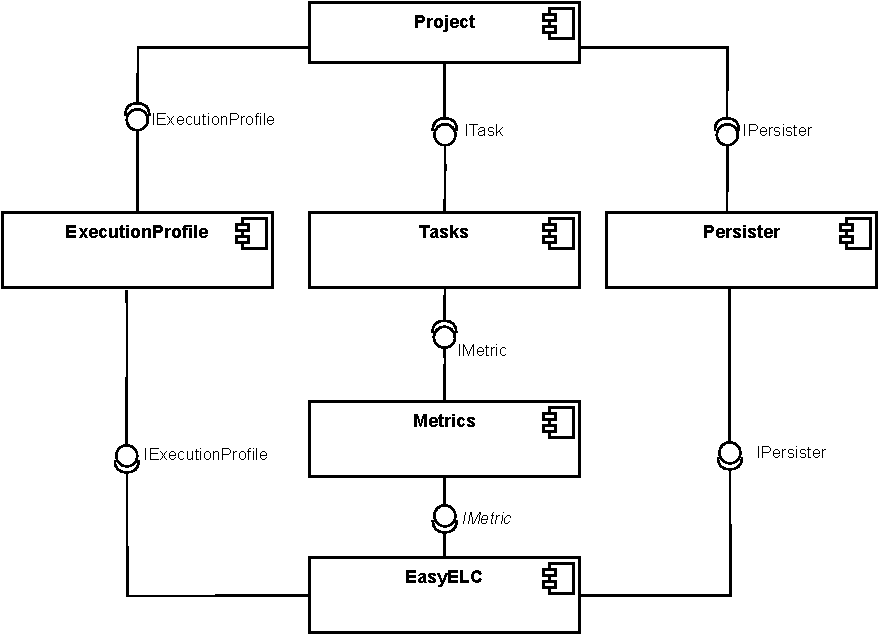
\includegraphics[width=0.6\textwidth]{figures/diagramaarquiteturaelchupacabra.pdf}
		\caption{Diagrama representando os relacionamentos entre os módulos internos da aplicação.}
		\label{fig:diagrama-arquitetura}
	\end{figure}


	\subsection{Módulo de Projeto (Project)}
	\label{subsection:modulo-project}

	O módulo de projeto é o módulo principal da ferramenta, onde o fluxo da coleta é iniciado. Ele é composto somente pela classe Project. O bloco de código \ref{lst:project_class} contém a classe criada para representar um projeto.

	\begin{lstlisting}[label={lst:project_class}, caption={Implementação da classe responsável por representar um projeto.}, language=TypeScript, breaklines=true]
	export default class Project {
	protected ExecutionProfile: IExecutionProfile;
	protected Persister: IPersister;
	protected Task: ITask;


	constructor(profile: IExecutionProfile, task: ITask, persister: IPersister) {
		this.ExecutionProfile = profile;
		this.Persister = persister;
		this.Task = task;
	}

	async executeTask(): Promise<void> {
		try {
			const profileData = await this.ExecutionProfile.collect();

			const result = await this.Task.run();

			await this.Persister.save({
				profile: profileData,
				taskResult: result,
			});
		} catch (error) {
			console.error("An error occurred during task execution:", error);
		}
	}
	}
	\end{lstlisting}

	Essa classe possui como atributos uma instância da classe ExecutionProfile, que contém as informações de quem está executando aquele projeto, uma instância da classe Persister, que é a classe responsável pela persistência de dados, e uma instância da classe Task, que é a tarefa mãe a ser executada.

	Possui também um único método, o método executeTask(), que coleta as informações da máquina através do ExecutionProfile, dá início a execução das tarefas associadas àquele projeto e persiste os resultados.

	\subsection{Módulo de Perfil de Execução (ExecutionProfile)}
	\label{subsection:modulo-execution-profile}

	A função principal desse módulo é permitir que o usuário consiga coletar informações a respeito do ambiente no qual estão sendo executadas as tarefas. Dessa forma, é possível não só diferenciar os voluntários após a coleta, mas também analisar os ambientes nos quais as tarefas foram executadas. Esse módulo consiste basicamente de uma interface, a IExecutionProfile, e de suas implementações concretas, que representam os tipos de ambientes nos quais as tarefas podem ser executadas. O bloco de código \ref{lst:execution_profile_abstract_class} a seguir contém a classe abstrata IExecutionProfile.

	\begin{lstlisting}[label={lst:execution_profile_abstract_class}, caption={Implementação da classe responsável por representar um perfil de execução.}, language=TypeScript, breaklines=true]
	export default interface IExecutionProfile {
		/**
		* Collects execution profile data.
		* @returns {Promise<Record<string, any>>} An object containing every execution profile data the
		* implementation was able to collect.
		*/
		collect(): Promise<Record<string, any>>;
	}
	\end{lstlisting}

	Essa interface contém os métodos collect(), que é o método que efetivamente coleta as informações do ambiente, e o método getVisitorId(), que provê um identificador único ao voluntário na execução para posterior análise. Ambos podem ser sobrescritos na implementação concreta de cada perfil, de acordo com a necessidade de cada ambiente.

	Supondo uma execução de tarefas em um navegador, deve ser implementada uma classe chamada BrowserExecutionProfile, que conteria as implementações concretas dos métodos para realizar a coleta dos dados do ambiente do navegador. O bloco de código \ref{lst:browser_execution_profile_abstract_class} a seguir contém a classe BrowserExecutionProfile.

	\begin{lstlisting}[label={lst:browser_execution_profile_abstract_class}, caption={Implementação da classe responsável por representar um perfil de execução.}, language=TypeScript, breaklines=true]
	export default class BrowserExecutionProfile implements IExecutionProfile {

	async collect(): Promise<Record<string, any>> {
		const date = new Date()
		const executionProfile: Record<string, any> = {
		software: {
			type: "Browser",
			userAgent: navigator.userAgent,
			language: navigator.language,
			windowInnerWidth: window.innerWidth,
			windowInnerHeight: window.innerHeight,
			devicePixelRatio: window.devicePixelRatio,
			appCodeName: window.navigator.appCodeName,
			appName: window.navigator.appName,
			appVersion: window.navigator.appVersion,
			product: window.navigator.product,
			productSub: window.navigator.productSub,
			vendor: window.navigator.vendor,
			vendorSub: window.navigator.vendorSub,
			doNotTrack: window.navigator.doNotTrack,
			isWebdriver: typeof window.navigator.webdriver !== 'undefined' ? window.navigator.webdriver.toString() : 'unknown'
		},
		os: {
			timeZoneOffset: date.getTimezoneOffset()
		},
		hardware: {
			screen: {
			width: screen.width,
			height: screen.height,
			colorDepth: screen.colorDepth,
			pixelDepth: screen.pixelDepth,
			},
			hardwareConcurrency: window.navigator.hardwareConcurrency
		},
		volatile: {
			localeDatetime: {
			date: date.toLocaleDateString(),
			time: date.toLocaleTimeString()
			},
			totalJSHeapSize: (window.performance as any).memory?.totalJSHeapSize || -1
		}
		}

		const fingerprintString = JSON.stringify(
		{
			software: executionProfile.software,
			os: executionProfile.os,
			hardware: executionProfile.hardware
		})
		executionProfile.visitorId = await this.getVisitorId(fingerprintString)

		return executionProfile
	}

	private async getVisitorId(input: string): Promise<string> {
		const encoder = new TextEncoder();
		const data = encoder.encode(input);
		const buffer = await crypto.subtle.digest('SHA-256', data);
		const hashArray = new Uint8Array(buffer);
		const hashHex = Array.from(hashArray)
		.map(byte => byte.toString(16).padStart(2, '0'))
		.join('');
		return hashHex;
	}
	}
	\end{lstlisting}

	\subsection{Módulo de Tarefas (Tasks)}
	\label{subsection:modulo-tasks}

	Esse módulo permite ao usuário implementar tarefas customizadas, sejam elas tarefas simples ou compostas (utilizando o padrão \hyperref[subsection:composite]{Composite}), e também permite a realização de processamentos pré e pós tarefa. Essas tarefas posteriormente são executadas pelo módulo principal de Project.
	Assim como o anterior, consiste de uma interface genérica (nesse caso a ITask) e suas implementações concretas. A classe exemplo para a criação de outras classes é a BaseTask, que traz a estrutura básica de uma tarefa, implementando a interface ITask. O bloco de código \ref{lst:basetask_class} a seguir contém a classe BaseTask.

	\begin{lstlisting}[label={lst:basetask_class}, caption={Implementação da classe responsável por representar uma tarefa básica.}, language=TypeScript, breaklines=true]
	export default abstract class BaseTask implements ITask {
	protected metrics: IMetric[]

	/**
		* Base constructor for all Tasks.
		* @param {IMetric[]} metrics - Metrics to be collected from this task.
		*/
	constructor(metrics: IMetric[]) {
		this.metrics = metrics
	}

	/**
		* @inheritdoc
		*/
	async run(): Promise<Record<string, any>> {
		await this.preTaskJob()
		this.metrics.forEach(x => x.start())
		const result = await this.execute()

		result.metrics = {}
		this.metrics.forEach(async x => {
		result.metrics[x.constructor.name] = await x.collect()
		})
		await this.postTaskJob()

		return { [this.constructor.name]: result }
	}

	/**
		* Executes the task with metric collection.
		* @abstract
		* @returns {Promise<Record<string, any>>} A promise that resolves with a report containing
		* metrics and data about the task execution.
		*/
	protected abstract execute(): Promise<Record<string, any>>

	/**
		* Override this method to perform pre-task jobs.
		* @protected
		*/
	protected async preTaskJob(): Promise<void> {
		return Promise.resolve()
	}

	/**
		* Override this method to perform post-task jobs.
		* @protected
		*/
	protected async postTaskJob(): Promise<void> {
		return Promise.resolve()
	}
	}
	\end{lstlisting}

	A interface ITask contém três métodos principais, que permitem ao usuário criar sua tarefa customizada. O primeiro é o método principal run(), no qual é inserido a chamada para a execução dos jobs e das métricas. Após isso, também são declarados os métodos preTaskJob e postTaskJob, os quais respectivamente representam as execuções que devem rodar antes e depois da tarefa.

	A tarefa aqui pode ser desde a transferência de um arquivo, até a execução de uma consulta em um banco de dados. Respeitando a interface principal, podem ser inseridos n tipos de tarefas diferentes, de acordo com a necessidade do usuário. Cada tarefa contém um conjunto de métricas, que são as representações dos tipos de dados que serão coletados na execução daquela tarefa.

	Quando houver a demanda de uma tarefa composta por mais de uma tarefa, a implementação se dá utilizando o padrão Composite (citar fundamentação teórica), e a tarefa passa a conter uma lista de tarefas associadas. Assim, quando o método run() é chamado na tarefa mãe, é feita uma iteração nas tarefas associadas para a execução em cadeia de todas as tarefas. O bloco de código \ref{lst:compositetask_class} a seguir contém a classe CompositeTask, que estende a BaseTask e representa uma tarefa composta.

	\begin{lstlisting}[label={lst:compositetask_class}, caption={Implementação da classe responsável por representar uma tarefa composta.}, language=TypeScript, breaklines=true]

	export default class CompositeTask extends BaseTask {
		private tasks: ITask[]
		private childTaskNamesMap: Record<string, Array<string>>

		constructor(metrics: IMetric[], tasks: ITask[]) {
			super(metrics)
			this.tasks = tasks
			this.childTaskNamesMap = this.generateChildTaskNamesMap(tasks)
		}

		protected async execute(): Promise<Record<string, any>> {
			const results: Record<string, any> = {}

			for (const task of this.tasks) {
				let taskResult = await task.run()
				let key = this.childTaskNamesMap[task.constructor.name].shift() || task.constructor.name
				results[key] = taskResult[task.constructor.name]
			}

			return results
		}

		private generateChildTaskNamesMap(tasks: ITask[]): Record<string, Array<string>> {
			const namesMap: Record<string, Array<string>>  = {}

			tasks.map(x => {
				const taskName = x.constructor.name

				if (!(taskName in namesMap)) {
					namesMap[taskName] = [`${taskName}_0`]
				}
				else {
					namesMap[taskName].push(`${taskName}_${namesMap[taskName].length}`)
				}
			})
			
			return namesMap
		}
	}

	\end{lstlisting}


	\subsection{Módulo de Métricas (Metrics)}
	\label{subsection:modulo-metrics}

	O módulo de métricas (Metrics) tem como objetivo representar as métricas que serão coletadas pela ferramenta. Essas métricas estão contidas nas tarefas (Tasks), e são elas as responsáveis de efetivamente coletar o dado desejado do ambiente no qual está sendo executada a tarefa. Esse módulo, assim como os anteriores, consiste de uma interface genérica (nesse caso a interface IMetric) e de suas implementações concretas. O bloco de código \ref{lst:imetric_abstract_class} a seguir contém a classe abstrata IMetric.

	\begin{lstlisting}[label={lst:imetric_abstract_class}, caption={Implementação da classe responsável por representar uma métrica.}, language=TypeScript, breaklines=true]
	/**
	* Represents a contract for collecting an execution metric.
	* @interface
	*/
	export default interface IMetric {
		/**
		* Marks the start of the profiling for the metric.
		*/
		start(): void;

		/**
		* Collects data related to the execution metric.
		* @returns {Promise<Record<string, any>>} A record containing the collected metric data.
		*/
		collect(): Promise<Record<string, any>>;
	}
	\end{lstlisting}

	A interface principal contém somente um método chamado collect(), que é responsável por executar a coleta efetiva do dado desejado. Estendendo essa interface, a implementação concreta sobrescreve esse método inserindo nele os processamentos necessários para a coleta. Esse método é chamado posteriormente para cada uma das métricas associadas na execução de uma tarefa. O bloco de código \ref{lst:memorymetric_class} a seguir contém um exemplo de implementação de métrica, a classe MemoryMetric.

	\begin{lstlisting}[label={lst:memorymetric_class}, caption={Implementação da classe responsável por representar uma métrica de memória.}, language=TypeScript, breaklines=true]

	export default class MemoryMetric implements IMetric {
	start(): void {
		return
	}

	async collect(): Promise<Record<string, any>> {
		const memoryConsumption = { usedApis: [] as string[], measurements: {} }
		const measurements = [
		await this.getNewBrowserApiMemoryData(),
		this.getOldBrowserApiMemoryData(),
		this.getNodeMemoryData()
		]

		for (let m of measurements) {
		if (Object.keys(m).length === 0) {
			continue
		}

		memoryConsumption.usedApis.push(Object.keys(m)[0])
		memoryConsumption.measurements = { ...memoryConsumption.measurements, ...m }
		}

		return memoryConsumption
	}

	private async getNewBrowserApiMemoryData(): Promise<Record<string, any>> {
		try {
		if (!self.crossOriginIsolated) {
			Promise.resolve({})
		}

		return {
			["measureUserAgentSpecificMemory"]: {
			memory: await (performance as any).measureUserAgentSpecificMemory()
			}
		}
		}
		catch {
		return Promise.resolve({})
		}
	}

	private getOldBrowserApiMemoryData(): Record<string, any> {
		try {
		const memoryInfo = (performance as any).memory;
		return {
			["performance.memory"]: {
			usedJSHeapSize: memoryInfo.usedJSHeapSize,
			totalJSHeapSize: memoryInfo.totalJSHeapSize,
			jsHeapSizeLimit: memoryInfo.jsHeapSizeLimit
			}
		}
		}
		catch {
		return {}
		}
	}

	private getNodeMemoryData(): Record<string, any> {
		try {
		const memoryUsage = process.memoryUsage()
		return {
			["process.memoryUsage"]: {
			rss: memoryUsage.rss,
			heapTotal: memoryUsage.heapTotal,
			heapUsed: memoryUsage.heapUsed
			}
		}
		}
		catch {
		return {}
		}
	}
	}
	\end{lstlisting}


	\subsection{Módulo de Persistência (Persister)}
	\label{subsection:modulo-persister}

	O módulo de persistência (Persister) tem como finalidade encapsular a persistência de dados após a coleta das métricas, a fim de facilitar o uso de diferentes formas de persistência de dados no contexto do framework. Dessa forma, é possível adaptar facilmente a implementação da persistência sem interferir na estrutura das tarefas. Esse módulo é composto pela interface genérica IPersister e suas implementações concretas, assim como os anteriores. O bloco de código \ref{lst:ipersister_abstract_class} a seguir contém a classe abstrata IPersister.

	\begin{lstlisting}[label={lst:ipersister_abstract_class}, caption={Implementação da classe responsável pela persistência dos dados.}, language=TypeScript, breaklines=true]
	/**
	* Represents a contract for persisting data.
	* @interface
	*/
	export default interface IPersister {
		/**
		* Saves data to a persistent storage.
		* @param {Record<string, any>} data - The data to be saved.
		* @returns {Promise<void>} A promise that resolves when the data is saved.
		*/
		save(data: Record<string, any>): Promise<void>;
	}
	\end{lstlisting}

	A interface é composta somente por um método chamado save(), no qual é realizada a persistêcia dos dados propriamente dita. Desse modo, ao instanciar um novo Persister, é nesse método que são realizados os processamentos necessários para salvar o dado da forma desejada. No bloco de código \ref{lst:sheetson_class} segue um exemplo de implementação da classe utilizada no exemplo proposto na seção X, o SheetsonPersister.

	\begin{lstlisting}[label={lst:sheetson_class}, caption={Implementação da classe responsável pela persistência dos dados usando o Sheetson.}, language=TypeScript, breaklines=true]

	export default class SheetsonPersister implements IPersister {
	private apiUrl: string;
	private apiKey: string;
	private spreadsheetId: string;

	constructor(apiUrl: string, apiKey: string, spreadsheetId: string) {
		this.apiUrl = "https://api.sheetson.com/v2/sheets/" + apiUrl;
		this.apiKey = apiKey;
		this.spreadsheetId = spreadsheetId;
	}

	async save(data: Record<string, any>): Promise<void> {
		try {
		const flattenData = Flatten.flatten(data, { delimiter: '.', safe: true });
		console.log(Object.keys(flattenData).join('\n'));
		
		const response = await fetch(this.apiUrl, {
			method: 'POST',
			headers: {
			'Content-Type': 'application/json',
			'Authorization': `Bearer ${this.apiKey}`,
			'X-Sheetson-Spreadsheet-Id': this.spreadsheetId
			},
			body: JSON.stringify(flattenData, (_, value) => {
			if (!Array.isArray(value)) {
				return value
			}

			return JSON.stringify(value)
			})
		});

		if (!response.ok) {
			throw new Error(`Failed to save data: ${response.statusText}`);
		}

		} catch (error) {
		if (error instanceof Error) {
			throw new Error(`Error saving data: ${error.message}`);
		} else {
			throw new Error('An unknown error occurred while saving data.');
		}
		}
	}
	}
	\end{lstlisting}


	\subsection{Módulo da Interface de Uso Simplificada (EasyELC)}
		\label{subsec:implemencao-easyelc}

	O módulo EasyElc tem como principal objetivo simplificar o uso do framework quando ele for uma dependência de outro projeto.
	Um dos possíveis casos de uso para o \acr{ELC}, é quando os procedimentos a serem avaliados existem em um sistema grande e complexo com múltiplas dependências.
	Neste cenário, incluir o \acr{ELC} como uma dependência no sistema que executa suas avaliações com o mínimo de modificações é na prática um pré-requisito.
	Para isso, publicamos o \acr{ELC} como um pacote no \acr{NPM} onde seu principal fluxo de uso é por meio do módulo EasyElc.

	A principal classe do módulo também é EasyElc, a qual recebe as mesmas configurações que uma instância de Project \ref{subsection:modulo-project}.
	A instância do EasyElc possui apenas o método público startProfiling \ref{lst:easyelc_startprofiling}, responsável por iniciar uma avaliação.
	Ele recebe como parâmetros uma string que é utilizada como token de identificação daquela avaliação nos resultados e uma lista de métricas.
	Além disso, o método retorna um objeto que contém apenas um método finish, que finaliza aquela análise e recebe possíveis metadados para agregar nos resultados.

	O funcionamento do módulo consiste em construir uma árvore de Profilings \ref{lst:easyelc_profiling_class} a partir das chamadas de startProfiling.
	Uma chamada de startProfiling cria um nó na árvore, se uma nova chamada for feita antes do finish da anterior, então, o novo nó será um filho do nó anterior.
	Por fim, a persistência das métricas coletadas é realizada quando todos os nós da árvore tiverem seu método finish executado e depois a árvore é descartada.

	\begin{lstlisting}[label={lst:easyelc_startprofiling}, caption={Implementação do método startProfiling da classe EasyElc.}, language=TypeScript, breaklines=true]
	startProfiling(uniqueName: string, metrics: IMetric[]): Record<string, any> {
		const newProfiling = new Profiling(uniqueName, metrics);

		if (this._profilingsTree === null) {
			this._profilingsTree = newProfiling;
		}
		else {
			const parentNode = this._getNewestActiveProfiling() ?? this._profilingsTree;

			if (uniqueName in parentNode.childs) {
				const numberOfAppearences = Object.keys(parentNode.childs).filter(k => k.match(new RegExp(`^${uniqueName}(\$|_[0-9]{1,}\$`))).length
				parentNode.childs[`${uniqueName}_${numberOfAppearences}`] = newProfiling;
			}
			else {
				parentNode.childs[uniqueName] = newProfiling;
			}
		}
		
		this._activeProfilingsStack.push(newProfiling);
		metrics.forEach(x => x.start());
		return { finish: (metadata: Record<string, any> | null = null) => {
			newProfiling.metadata = metadata;
			this._terminateProfiling(newProfiling);
		} };
	}
	\end{lstlisting}

	\begin{lstlisting}[label={lst:easyelc_profiling_class}, caption={Implementação do nó da árvore de análises usado no EasyElc.}, language=TypeScript, breaklines=true]
	export default class Profiling {
		uniqueName: string;
		runningMetrics: IMetric[];
		metricsResults: Record<string, any>[];
		metadata: Record<string, any> | null;
		childs: Record<string, Profiling>;

		constructor(uniqueName: string, metrics: IMetric[]) {
			this.uniqueName = uniqueName;
			this.runningMetrics = metrics;
			this.metricsResults = [];
			this.metadata = null;
			this.childs = {};
		}
	}
	\end{lstlisting}



	\section{Diagrama de Casos de Uso}
	\label{sec:diagrama_de_caso_de_uso}

	O diagrama de casos de uso é o diagrama responsável por prever como a ferramenta será utilizada, embasando futuramente o desenvolvimento e os testes da aplicação. No caso do ELC, temos os atores ...

	\begin{figure}[!ht]
		\centering
		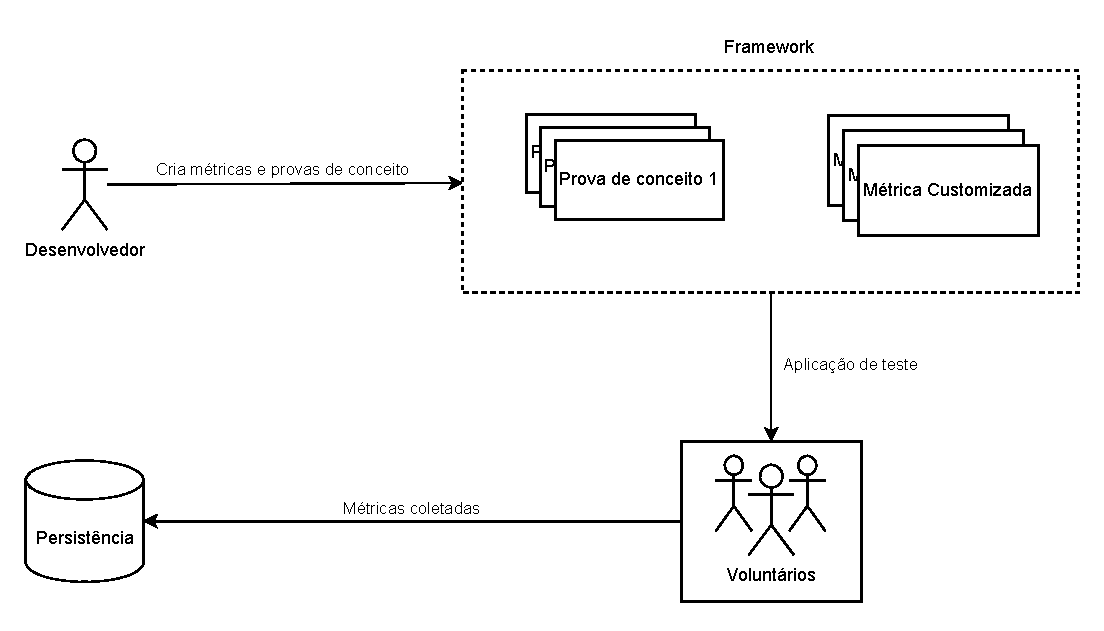
\includegraphics[width=0.6\textwidth]{figures/diagrama-informal.pdf}
		\caption{Principal fluxo de uso, onde um desenvolver avalia um conjunto de provas de conceitos com o auxílio de voluntários externos ao desenvolvimento.}
		\label{fig:diagrama-informal}
	\end{figure}

		
	\section{Diagrama de Classes}
	\label{cap:diagrama_de_classe}


	O diagrama conceitual detalhado define a arquitetura e estrutura dos módulos do framework.
	Nele há a definição dos principais aspectos práticos para a implementação, por exemplo, são definidas as árvores de herança e principais métodos que precisam ser implementados por usuários.
	Além disso, ele também define a camada de persistência para resolver o problema da coleta de métricas de execuções realizadas por voluntários de forma remota.
	Abaixo, está uma descrição de cada elemento do diagrama.

	\begin{figure}[!ht]
		\centering
		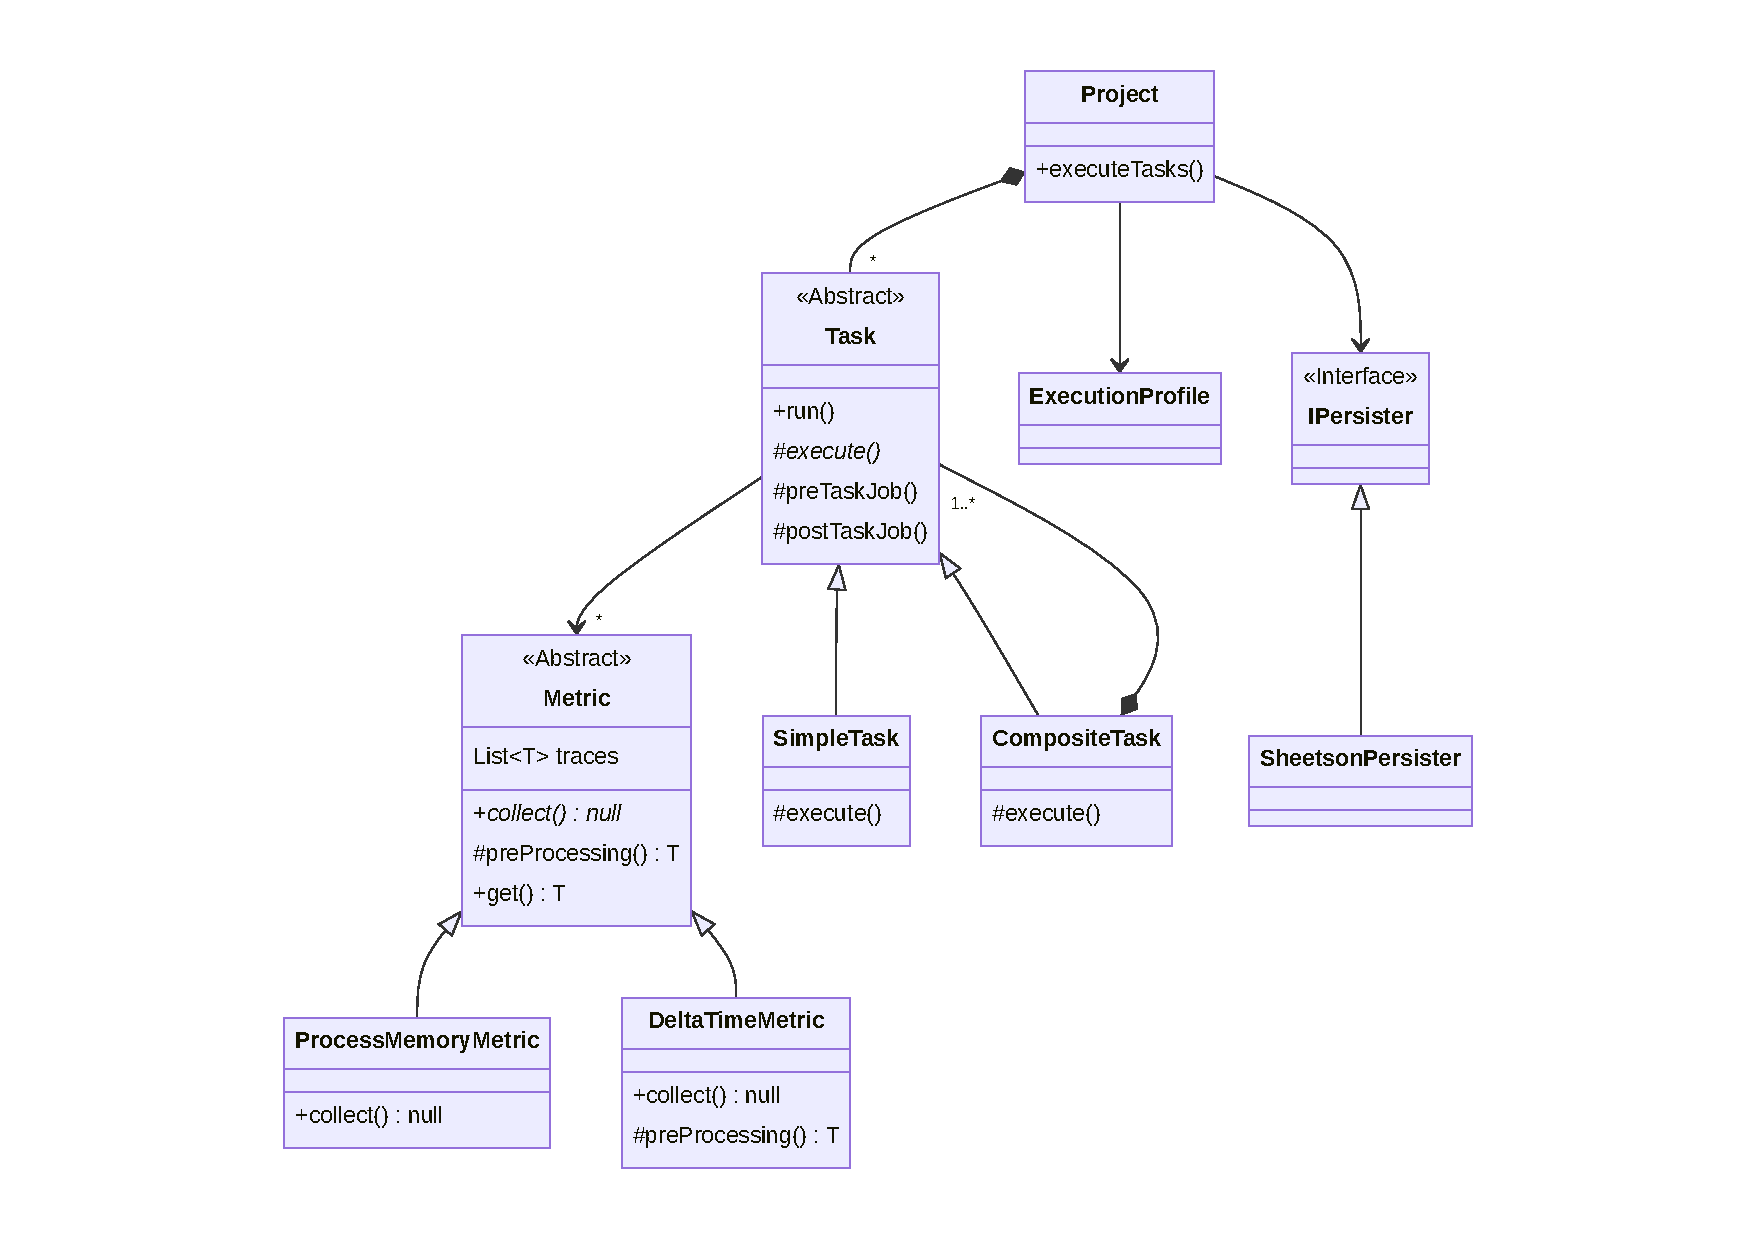
\includegraphics[width=0.9\textwidth]{figures/diagrama-classes.pdf}
		\caption{Diagrama conceitual detalhado do framework.}
		\label{fig:diag-classes}
	\end{figure}


	\begin{description}
		\item[Project:] Responsável por coordenar a execução das análises e encaminhar suas métricas para a camada de persistência.
		\item[ExecutionProfile:] Responsável pela coleta de dados sobre o ambiente de execução.
		\item[Task:] Responsável por definir a rotina de execução das tarefas e seus métodos públicos.
		\item[SimpleTask:] Classe base para implementação de uma tarefa.
		\item[CompositeTask:] Classe base para implementação de tarefas compostas.
		\item[Metric:] Responsável por definir a rotina para coleta de uma métrica e seus métodos públicos.
		\item[ProcessMemoryMetric:] Implementação de uma métrica para medir o consumo de memória.
		\item[DeltaTimeMetric:] Implementação de uma métrica para medir tempo gasto em uma tarefa.
		\item[IPersister:] Responsável por definir a interface pública da camada de persistência.
		\item[SheetsonPersister:] Implementação da camada de persistência a qual utiliza o Google Sheets\footnote{https://www.google.com/sheets/about}.
	\end{description}


\chapter{Experimentos}
	\label{cap:experimentos}

	Após o desenvolvimento do \acr{ELC}, é necessária a realização de um experimento para avaliar como se daria o seu uso em um cenário real. Neste capítulo estão contidas as descrições do experimento utilizado para avaliar o \acr{ELC} por voluntários externos, bem como sua preparação e execução. Além disso, estão contidos também os resultados do experimento.

	\section{Preparação do experimento}
	\label{section:preparacao-experimento}

	O experimento consiste em duas etapas principais. A primeira é a utilização do \acr{ELC} em um projeto exemplo, e a segunda é o preenchimento de um formulário no Google Forms baseado no \acr{SUS}, buscando coletar a opinião do voluntário de como foi a experiência de uso.

	Para o grupo de controle, estão sendo considerados XX voluntários, em sua maioria alunos e/ou pertencentes à comunidade do CEFET e já com alguma experiência em programação. 

	% TO-DO: Substituir número de voluntários

	\section{Uso do ELC pelos voluntários}
	\label{section:parte-1-experimento}


	% TO-DO: Revisar seção pra bater com o que está no observable


	A primeira parte do experimento consiste basicamente do uso do \acr{ELC}, mais especificamente do módulo EasyELC, pelos voluntários através da plataforma \emph{ObservableHQ}\footnote{Link para o experimento na plataforma ObservableHQ: https://observablehq.com/@moura/framework-el-chupacabra-experimento}. Um projeto padrão foi criado e disponibilizado para os voluntários, e consiste em comparar o desempenho de dois algoritmos de ordenação já conhecidos sobre um conjunto de dados. Os algoritmos são o Bubble Sort e o Heap Sort, e o conjunto de dados está inicialmente desordenado e representado no formato \acr{JSON}. Dessa forma, o fluxo do experimento a ser realizado é: realizar a ordenação duas vezes, uma utilizando cada algoritmo, para comparar qual tem o melhor desempenho.

	Foi adicionado uma seção chamada Implementação de Métrica Customizada, como mostra a figura \ref{fig:metrica-observable}. Essa parte do código é uma das partes que o voluntário preenche, com o auxílio de comentários deixados mostrando o passo a passo da criação da métrica. O exemplo trata de uma métrica cujo comportamento é retornar um número aleatório. Dessa forma, ele consegue ter a experiência de criar uma métrica utilizando a ferramenta.

	\begin{figure}[!ht]
		\centering
		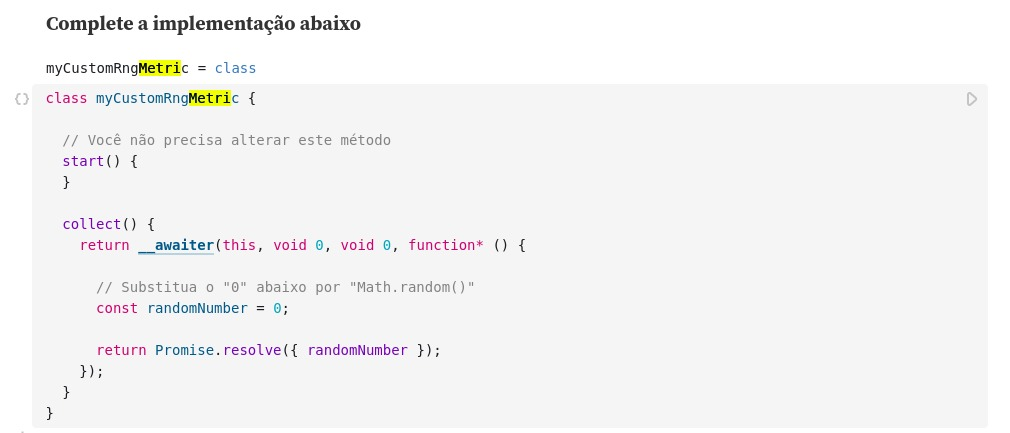
\includegraphics[width=1\textwidth]{figures/experimento-metrica.jpeg}
		\caption{Seção para criação de métrica customizada pelo usuário no experimento.}
		\label{fig:metrica-observable}
	\end{figure}


	Após a ordenação realizada pelo algoritmo, o \acr{ELC} é chamado para registrar quanto tempo durou a ordenação de todo o arquivo. O fluxo para o Bubble Sort está descrito na figura \ref{fig:experimento-bubble}, e para o Heap Sort na figura \ref{fig:experimento-heap}.

	\begin{figure}[!ht]
		\centering
		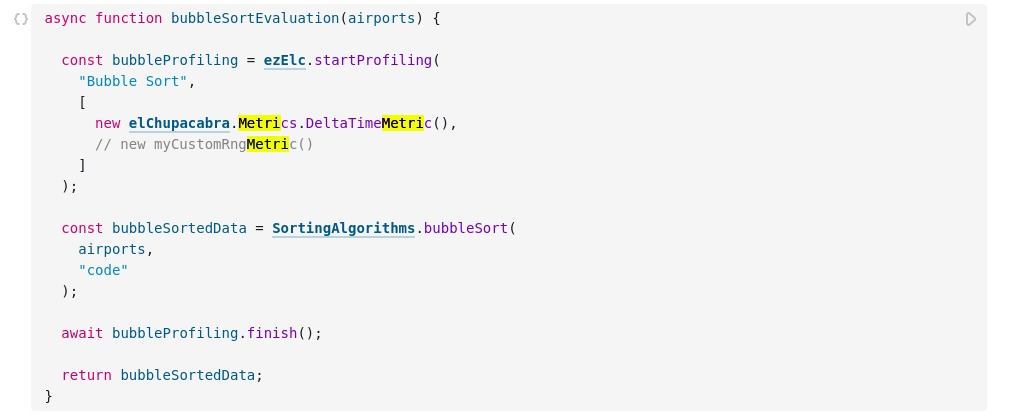
\includegraphics[width=1\textwidth]{figures/experimento-bubble.jpeg}
		\caption{Fluxo de código referente a execução da ordenação com o Bubble Sort.}
		\label{fig:experimento-bubble}
	\end{figure}

	\begin{figure}[!ht]
		\centering
		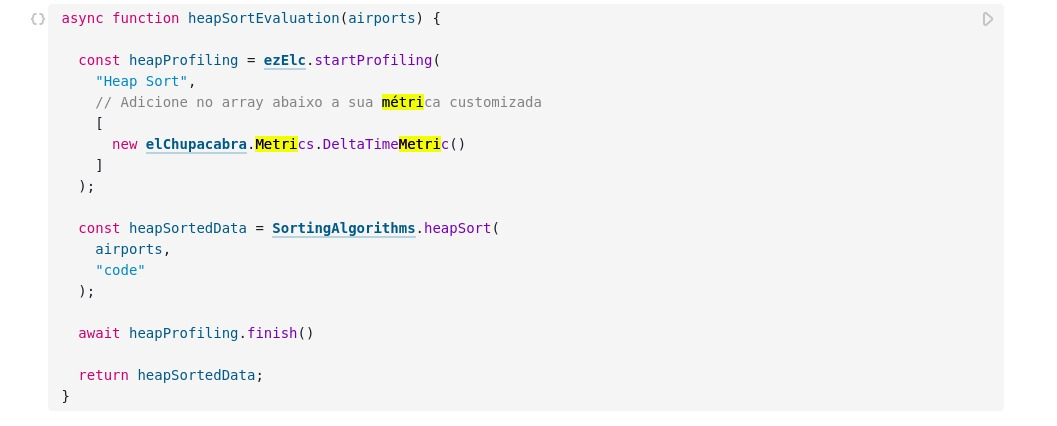
\includegraphics[width=1\textwidth]{figures/experimento-heap.jpeg}
		\caption{Fluxo de código referente a execução da ordenação com o Heap Sort.}
		\label{fig:experimento-heap}
	\end{figure}


	Os resultados da execução do experimento são inseridos em uma tabela no Google Sheets, como mostra a figura \ref{fig:experimento-tabela-resultado}, e disponibilizados para os voluntários verem como a inserção das métricas acontece. Assim, a primeira parte do experimento cobre todo o fluxo principal de execução do \acr{ELC}.

	\begin{figure}[!ht]
		\centering
		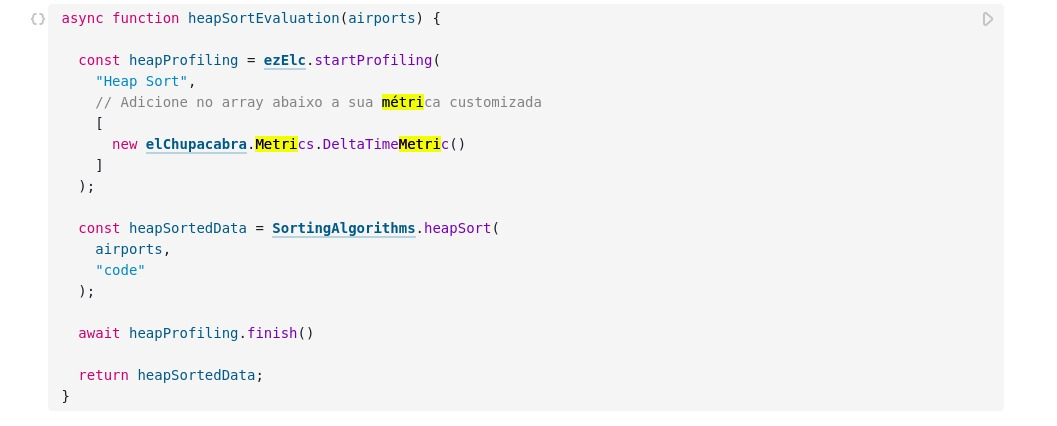
\includegraphics[width=1\textwidth]{figures/experimento-heap.jpeg}
		\caption{Seção para criação de métrica customizada pelo usuário no experimento.}
		\label{fig:experimento-tabela-resultado}
	\end{figure}


	\section{Formulário}
	\label{section:parte-2-formulario}

	Após a realização da primeira etapa do experimento, os voluntários preenchem um formulário, cujo objetivo é avaliar a experiência de uso da ferramenta, bem como outras características relevantes para a análise do seu desempenho e qualidade. As perguntas do formulário são baseadas no conceito trazido pelo \acr{SUS}. Esse sistema de avaliação foi construído para fornecer uma forma sólida e com baixo custo de implementação de avaliar a usabilidade de sistemas de software \citep{brooke1995sus}. Na lista abaixo estão as perguntas já traduzidas que são utilizadas no formulário.

	\begin{enumerate}
		\itemsep 0em 

		\item Eu acho que gostaria de usar esse sistema com frequência.
		\item Eu acho o sistema desnecessariamente complexo.
		\item Eu achei o sistema fácil de usar.
		\item Eu acho que precisaria de ajuda de uma pessoa com conhecimentos técnicos para usar o sistema.
		\item Eu acho que as várias funções do sistema estão muito bem integradas.
		\item Eu acho que o sistema apresenta muita inconsistência.
		\item Eu imagino que as pessoas aprenderão como usar esse sistema rapidamente.
		\item Eu achei o sistema atrapalhado de usar.
		\item Eu me senti confiante ao usar o sistema.
		\item Eu precisei aprender várias coisas novas antes de conseguir usar o sistema.
	\end{enumerate}


	\section{Resultados}
	\label{section:resultados}

	Na primeira parte do experimento, foi observada uma grande adesão por parte dos voluntários, e nenhum dos voluntários necessitou de ajuda para realizar a tarefa. Isso demonstra sucesso na utilização da ferramenta, e é um indício de que o \acr{ELC} não é uma ferramenta complicada de se utilizar no dia a dia.

	Na segunda parte do experimento, após a submissão dos formulários, é possível gerar um gráfico para cada pergunta contendo quais foram as respostas mais selecionadas pelos voluntários. Os resultados do formulário mostram que o \acr{ELC} conseguiu atingir um nível adequado de usabilidade em sua primeira versão, obtendo uma nota média de XX.


	% TO-DO: Substituir gráficos com resultados do google forms


	\begin{figure}[!ht]
		\centering
		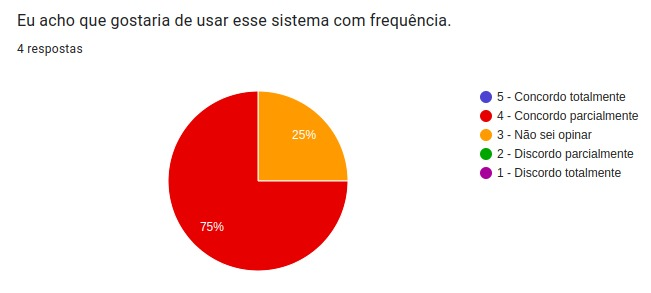
\includegraphics[width=0.8\textwidth]{figures/respostas-pergunta-1.jpeg}
		\caption{Respostas obtidas na pergunta 1}
		\label{fig:respostas-pergunta-1}
	\end{figure}

	\pagebreak

	\begin{figure}[!ht]
		\centering
		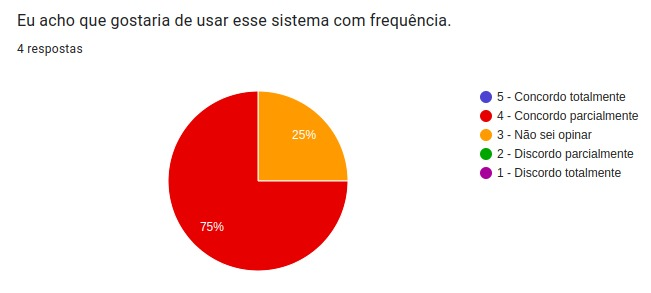
\includegraphics[width=0.8\textwidth]{figures/respostas-pergunta-2.jpeg}
		\caption{Respostas obtidas na pergunta 2}
		\label{fig:respostas-pergunta-2}
	\end{figure}

	\begin{figure}[!ht]
		\centering
		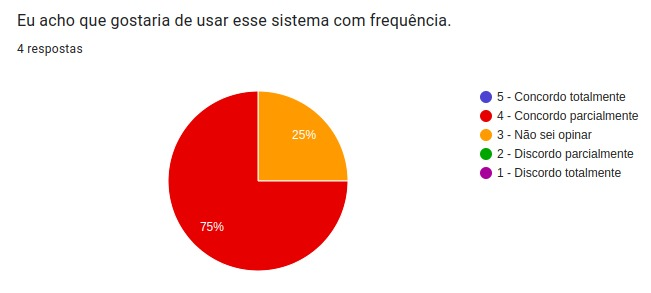
\includegraphics[width=0.8\textwidth]{figures/respostas-pergunta-3.jpeg}
		\caption{Respostas obtidas na pergunta 3}
		\label{fig:respostas-pergunta-3}
	\end{figure}

	\begin{figure}[!ht]
		\centering
		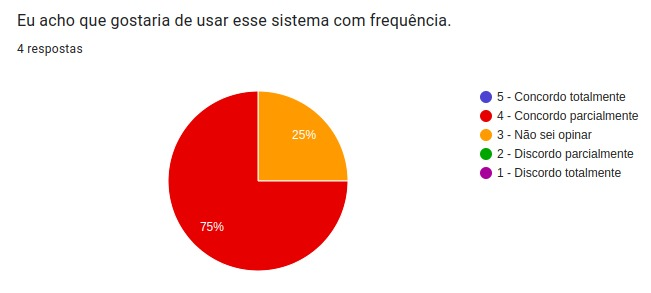
\includegraphics[width=0.8\textwidth]{figures/respostas-pergunta-4.jpeg}
		\caption{Respostas obtidas na pergunta 4}
		\label{fig:respostas-pergunta-4}
	\end{figure}

	\begin{figure}[!ht]
		\centering
		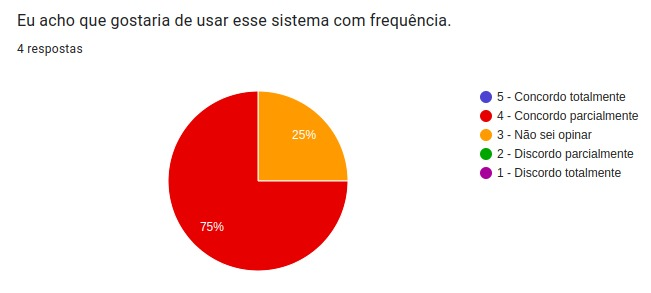
\includegraphics[width=0.8\textwidth]{figures/respostas-pergunta-5.jpeg}
		\caption{Respostas obtidas na pergunta 5}
		\label{fig:respostas-pergunta-5}
	\end{figure}

	\begin{figure}[!ht]
		\centering
		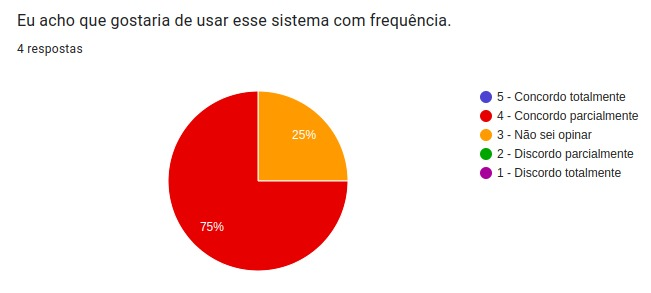
\includegraphics[width=0.8\textwidth]{figures/respostas-pergunta-6.jpeg}
		\caption{Respostas obtidas na pergunta 6}
		\label{fig:respostas-pergunta-6}
	\end{figure}

	\begin{figure}[!ht]
		\centering
		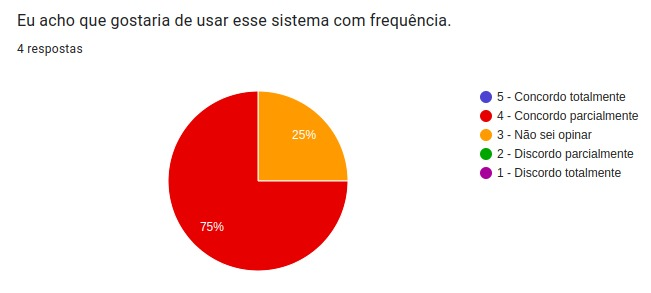
\includegraphics[width=0.8\textwidth]{figures/respostas-pergunta-7.jpeg}
		\caption{Respostas obtidas na pergunta 7}
		\label{fig:respostas-pergunta-7}
	\end{figure}


	\begin{figure}[!ht]
		\centering
		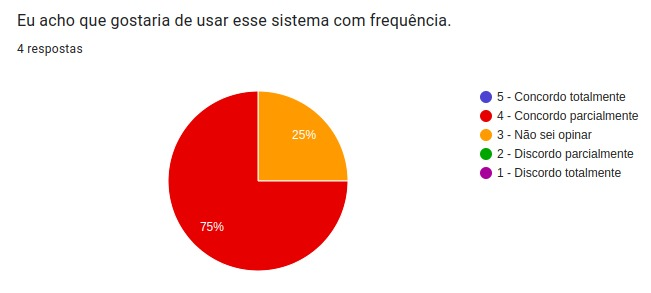
\includegraphics[width=0.8\textwidth]{figures/respostas-pergunta-8.jpeg}
		\caption{Respostas obtidas na pergunta 8}
		\label{fig:respostas-pergunta-8}
	\end{figure}

	\begin{figure}[!ht]
		\centering
		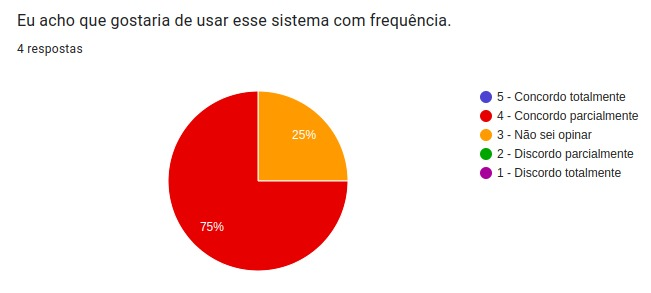
\includegraphics[width=0.8\textwidth]{figures/respostas-pergunta-9.jpeg}
		\caption{Respostas obtidas na pergunta 9}
		\label{fig:respostas-pergunta-9}
	\end{figure}

	\begin{figure}[!ht]
		\centering
		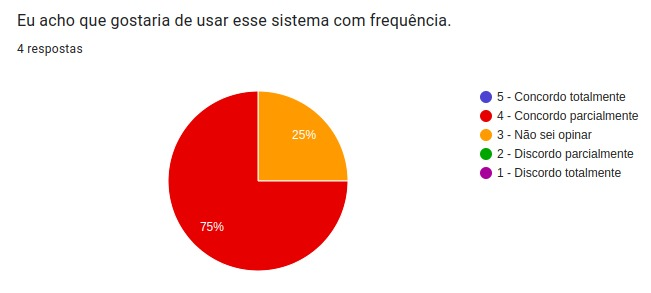
\includegraphics[width=0.8\textwidth]{figures/respostas-pergunta-10.jpeg}
		\caption{Respostas obtidas na pergunta 10}
		\label{fig:respostas-pergunta-10}
	\end{figure}

\chapter{Conclusão}
	\label{cap:conclusão}

	Neste capítulo estão contidas as conclusões obtidas após o projeto, implementação e experimentação da ferramenta. Assim, na seção \ref{section:analise-do-elc}, o \acr{ELC} foi comparado com as outras ferramentas encontradas, e classificado de acordo com os critérios estabelecidos anteriormente. Além disso, na seção \ref{section:trabalhos-futuros}, foram apontadas as limitações principais da ferramenta. Por fim, na seção \ref{section:trabalhos-futuros}, foram trazidas possibilidades para trabalhos futuros envolvendo o framework, a fim de aprimorá-lo.

	\section{Análise do ELC}
	\label{section:analise-do-elc}

	Após a experimentação da ferramenta, é possível posicioná-la com relação aos critérios que foram estabelecidos na seção \ref{sec:ferramentas-medicao-clientside}. O resultado da comparação com as outras ferramentas se encontra na tabela \ref{table:classificacao-com-elc}.

	\begin{table}[ht]
	\caption{Classificação das ferramentas encontradas com o ELC} % title of Table
	\centering % used for centering table
	\begin{tabular}{c c c c c c} % centered columns (4 columns)
	\toprule %inserts double horizontal lines

	\textbf{Ferramentas} &\textbf{MemInsight} & \textbf{WePR} & \textbf{Gember} & \textbf{Mobilyzer} & \textbf{ELC}  \\ [0.4ex]

	%heading
	\midrule % inserts single horizontal line
	Coesão e Acoplamento & \cmark & \cmark & \cmark & \cmark  & \cmark  \\ 
	Extensibilidade & \xmark & \xmark & \xmark & \xmark  & \cmark \\
	Portabilidade & \cmark & \xmark & \xmark & \xmark  & \cmark \\
	Armazenamento em núvem & \xmark & \cmark & \cmark & \cmark & \cmark  \\
	\bottomrule %inserts single line
	\end{tabular}
	\label{table:classificacao-com-elc} % is used to refer this table in the text
	\end{table}

	Voltando ao exemplo do grupo de pesquisadores desenvolvendo uma aplicação web, que foi trazido no começo deste trabalho, o \acr{ELC} não exige que o código fonte das provas de conceito sejam alterados para a sua utilização. Através da modelagem das tarefas e métricas, é possível realizar um experimento utilizando o código das provas de conceito como foram implementados inicialmente, apenas inserindo chamadas dentro das tarefas do \acr{ELC}. Assim, podem ser executadas diversas tarefas diferentes, mas na mesma estrutura e portanto com seus resultados registrados na mesma base de dados para análise. Isso significa que a aplicação da ferramenta no exemplo gera código com um nível bom de coesão e baixo de acoplamento, atendendo ao critério estabelecido de Coesão e Acoplamento. 

	Além disso, o \acr{ELC} tem uma arquitetura extensível, tanto na parte de métricas e tarefas já citadas, quanto nas partes de perfis de execução e persistência. É possível utilizar diversos tipos de bases de dados, seja o Sheetson, como foi exemplificado, ou um banco de dados. Basta estender a interface do Persister e implementar suas particularidades. Dessa forma, a ferramenta atende ao critério de Extensibilidade.

	Como o \acr{ELC} é executado no navegador, é possível executar medições em diversos dispositivos diferentes, sem problemas de compatibilidade, já que a execução é no próprio navegador. Além da métrica escolhida pelo pesquisador, é possível registrar também juntamente qual foi o aparelho que a executou e suas informações básicas, atendendo à experimentos multiplataforma que precisam dessas informações. Portanto, é possível dizer que a ferramenta atende ao critério de Portabilidade.

	No armazenamento das informações, o \acr{ELC} também atende aos requisitos por ser bastante extensível. Como dito anteriormente, no trabalho foi utilizado o Sheetson, uma ferramenta para habilitar a escrita de dados em planilhas do Google via \acr{API}, mas podem ser utilizados diversos tipos de bases de dados, como bancos de dados Postgresql e MongoDB. Assim, conclui-se que a ferramenta também atende ao critério de Armazenamento em Núvem.


	\section{Limitações do ELC}
	\label{section:limitacoes-elc}

	Como dito anteriormente, existem algumas limitações com relação ao uso do \acr{ELC}. A primeira delas é que só podem ser realizados hoje testes de caixa preta, ou seja, testes que utilizem dados obtidos durante a execução do programa. Isso limita um pouco o uso da ferramenta para alguns cenários, principalmente para testes de caixa branca \footnote{Sobre testes de caixa branca: \citep[Capítulo 21]{Sommerville2015Software}}, já que não pode ser utilizada para testes estáticos, como por exemplo para testar uma implementação de uma classe.

	\section{Trabalhos Futuros}
	\label{section:trabalhos-futuros}

	Como possibilidades de trabalhos futuros, é possível trazer o conceito de testes de caixa branca para a ferramenta. Dessa forma, o \acr{ELC} ficaria ainda mais robusto, abrangendo mais cenários de teste e contextos onde pode ser utilizado. Além disso, pode ser realizado mais um experimento, dessa vez contemplando o uso mais completo do \acr{ELC}, clonando diretamente do repositório. Esse experimento exige um rigor maior em sua estrutura, construção, e também necessita de voluntários mais experientes, além de precisar de mais tempo para ser realizado.


	\label{bibpage}
	\renewcommand\bibname{Referências}
	\addcontentsline{toc}{section}{Referências}
	\bibliography{references}
	%\bibliographystyle{plainnat}
	\bibliographystyle{apalike}
	\label{bibfinalpage}

	\label{lastpage}



	\appendix








\chapter{Prova de Conceito}
\label{apx:mock}

\section{Prova de conceito}
\label{cap:prova_de_conceito}

A fim de testar a modelagem proposta, desenvolvemos uma prova de conceito com objetos mock, os quais simulam recursos computacionais.
De modo que fosse possível avaliar a eficácia da modelagem sem depender de recursos reais, visando manter o foco em avaliar a estrutura do framework.
A prova de conceito foi implementada usando a linguagem de programação Typescript, sua escolha almeja expressar com clareza todas as classes e relações definidas durante a modelagem, e seu código-fonte pode ser encontrado no apêndice \ref{apx:mock_source}.


\subsection{Simulação de Recursos Computacionais}
Como mencionado anteriormente, a prova de conceito possui classes para simular recursos computacionais.
As quais possuem a finalidade de isolar a prova de conceito de complexidades inerentes a realização de medições reais.
Logo, o desenvolvimento da prova de conceito pode ser concentrado em explorar o ponto central da modelagem, a árvore de \emph{Tarefas}.
O bloco de código \ref{lst:mock_memoria} contém a classe criada para simular o consumo de memória.

\begin{lstlisting}[label={lst:mock_memoria}, caption={Implementação da classe responsável por simular recursos de memória para a prova de conceito do framework.}, language=TypeScript]
class Resource {
	private static _total: number = 500;

	static alloc(size: number): any {
		this._total -= size;
		return {size};
	}

	static free(block: any): void {
		this._total += block.size;
	}

	static get total(): number {
		return this._total;
	}
}
\end{lstlisting}


\subsection{Árvore de Tarefas}
\label{task-tree}

A árvore de tarefas é definida basicamente por três classes:
a classe abstrata \emph{Task}, responsável por definir o que uma tarefa faz, ou seja, a sua interface pública.
A classe \emph{CompositeTask}, a qual possui a função de agregar outras tarefas.
E, a classe \emph{SimpleTask}, responsável por encapsular e executar o código do usuário do framework.
Entretanto, tanto \emph{CompositeTask} quanto \emph{SimpleTask} servem apenas para fins de herança e polimorfismo.
Portanto, com o framework em sua completude, as derradeiras classes as quais compõem a árvore de tarefas, serão subclasses.

\begin{lstlisting}[label={lst:abstract_task}, caption={Classe abstrata responsável por definir o que todos os membros da árvore de tarefas precisam implementar.}, language=TypeScript]
abstract class Task {
	public name: string;
	public metrics: Set<Metric<any>>;

	constructor(name: string, metrics: Metric<any>[])
	{
		this.metrics = new Set(metrics);
		this.name = name;
	}

	async run(): Promise<any> {
		this.preTaskJob();
		let data = await this.execute();
		let metrics = {};
		this.metrics.forEach(element => {
		metrics[element.name] = element.metric;
		});
		this.postTaskJob();
		return {metrics, data};
	}

	preTaskJob(): void {};
	abstract execute(): Promise<any>;
	postTaskJob(): void {};
}
\end{lstlisting}

\begin{lstlisting}[label={lst:composite_task}, caption={Tarefa composta, define o comportamento de todos os nós não folha da árvore de tarefas.}, language=TypeScript]
export class CompositeTask extends Task {
	private tasks: Task[];

	constructor() {
		super("Composite Task", []);
		this.tasks = [];
	}

	addTask(task: Task): void {
		this.tasks.push(task);
		task.metrics.forEach(element => {
			this.metrics.add(element);
		});
	}

	async execute(): Promise<any> {
		console.log("Executing composite task...");
		let tasks = {};
		for (const task of this.tasks) {
			tasks[task.name] = await task.run();
		}
		return tasks;
	}
}
\end{lstlisting}


\subsection{Executando a Prova de Conceito}
\label{sec:exe_poc}
A fim de executar a prova de conceito, é necessário criar um arquivo o qual atua como roteiro principal, guiando a execução de outras partes do código.
Além disso, neste mesmo arquivo, é onde construímos a árvore de tarefas.
Ou seja, instanciamos tanto as tarefas compostas quanto às tarefas simples e estabelecemos a sua estrutura de árvore.
Por fim, também é instanciado um objeto \emph{Project} o qual recebe como parâmetros a raiz da árvore de tarefas e uma implementação da interface de persistência.

\begin{lstlisting}[label={lst:index_ts}, caption={Exemplo de roteiro principal para executar a prova de conceito.}, language=TypeScript]
class Index {
	public static async main() {
		console.log("Hello world!");
		const task = new CompositeTask();
		const task2 = new CompositeTask();
		task.addTask(new MockTask("Task 1"));
		task.addTask(new MockTask("Task 2"));
		task2.addTask(new MockTask("Task 3"));
		task.addTask(task2);
		const project = new Project(
			new BasicPersister(),
			task);
		project.executeTask();
	}
}
\end{lstlisting}


\appendix
\chapter{Código-fonte da Prova de Conceito}
\label{apx:mock_source}

\section{Projeto}
\lstinputlisting[language=TypeScript]{./mock/Project.ts}

\section{Index}
\lstinputlisting[language=TypeScript]{./mock/Index.ts}

\section{Tarefa Abstrata}
\lstinputlisting[language=TypeScript]{./mock/Tasks/Task.ts}

\section{Tarefa Composta}
\lstinputlisting[language=TypeScript]{./mock/Tasks/CompositeTask.ts}

\section{Tarefa Simples}
\lstinputlisting[language=TypeScript]{./mock/Tasks/SimpleTask.ts}

\section{Exemplo de implementação de tarefa}
\lstinputlisting[language=TypeScript]{./mock/Tasks/MockTask.ts}

\section{Interface de persistencia}
\lstinputlisting[language=TypeScript]{./mock/Persister/IPersister.ts}

\section{Exemplo de persistencia}
\lstinputlisting[language=TypeScript]{./mock/Persister/BasicPersister.ts}

\section{Mock de tempo}
\lstinputlisting[language=TypeScript]{./mock/Helpers/MockTime.ts}

\section{Mock de Memoria}
\lstinputlisting[language=TypeScript]{./mock/Helpers/MockResource.ts}

\section{Metrica abstrata}
\lstinputlisting[language=TypeScript]{./mock/Metrics/Metric.ts}

\section{Metrica de tempo}
\lstinputlisting[language=TypeScript]{./mock/Metrics/GetDeltaTime.ts}

\section{Metrica de memoria}
\lstinputlisting[language=TypeScript]{./mock/Metrics/GetResourceUsage.ts}

\end{document}